\documentclass[12pt]{article}
\usepackage{graphics}
\usepackage{psfig}
\oddsidemargin 6mm
\evensidemargin 6mm
\topmargin -6mm
\textwidth 165mm
\textheight 250mm
\headheight 5mm
\headsep 4mm
\parskip 4mm
\parindent 0em


\newcommand{\ie}{ {\em i.e. }}
\newcommand{\eg}{ {\em e.g. }}
\newcommand{\kms}{\mbox{km s$^{-1}$ }}
\newcommand{\cmt}{\mbox{cm$^{-3}$ }}
\newcommand{\um}{$\mu $m }
\newcommand{\degree}{^\circ}

\begin{document}

\pagestyle{empty}
\centering
\vspace*{2cm}

{\Huge\bf ASTROPHYSICS \\ Junior Honours
\vspace*{3mm}

 Lab Handbook}
\vspace*{1cm}

{\Huge\bf 2012/13}
\vspace*{1cm}

\scalebox{0.3}{\includegraphics{crest.eps}}
\vspace*{3cm}

{\huge\bf Spectroscopy

Astronomical Exercises


}

~
\newpage

\centering
{\Large\bf CONTENTS}
\vspace*{4cm}

\raggedright

{\bf
LAB TIMETABLE

REPORTS FORMAT

SPECTROSCOPY \\
\hspace*{2cm} Aims and Safety \\
\hspace*{2cm} Equipment inventory\\
\hspace*{2cm}1.  Adjustment of the prism spectrometer\\
\hspace*{2cm}2. Adjustment of the grating spectrometer\\
\hspace*{2cm}3. Identifying an unknown element\\
\hspace*{2cm}4. Calibrating a colour filter 

ASTRONOMICAL EXERCISES \\
\hspace*{2cm}1. CCD photometry\\
\hspace*{2cm}2. Quasar redshift \\
\hspace*{2cm}3. Astrometry of asteroids on Schmidt plates


APPENDIX 1:\ \ \ {\large\sl A CCD Atlas of Helium/Neon/Argon Spectra}\\
APPENDIX 2:\ \ \ {\large\sl Basic Unix Commands/Useful Software}\\
APPENDIX 3:\ \ \ {\large\sl Gnuplot tutorial}\\
APPENDIX 4:\ \ \ {\large\sl Error Propagation}\\
\vspace*{4cm}

%{\small\sl
%Edited expanded and revised by PWJL Brand.
%contributions (Quasar Redshift, 
%revision of Astrometry) by JS Dunlop. 
%Based on a programme developed by MJ Smyth and MT Br\"{u}ck from laboratory
%exercises devised by EA Baker. Thanks to
%Starlink Project of PPARC for software and documentation, and to J. Carder
%for his spectral atlas.
%}

\noindent
Last updated: 27/10/2012 by R. McLure


}

\newpage


%\begin{flushright}{\scriptsize Version 1}\end{flushright}

%\begin{center}
\begin{center}
{\Large {\bf Astrophysics 3 Laboratory Timetable\ \ 2012-13}}\\

\bigskip

\begin{tabular}{|c|ccccc||ccccccccc|}\hline
{{\scriptsize\bf Mon/Thu (Sem1)}} &
 $\stackrel{\mbox{\tiny 29}}{\mbox{\tiny Oct}}$ &
 $\stackrel{\mbox{\tiny  5}}{\mbox{\tiny Nov}}$ &
 $\stackrel{\mbox{\tiny 12}}{\mbox{\tiny Nov}}$ &
 $\stackrel{\mbox{\tiny 19}}{\mbox{\tiny Nov}}$ &
 $\stackrel{\mbox{\tiny 26}}{\mbox{\tiny Nov}}$ &
 $\stackrel{\mbox{\tiny 17}}{\mbox{\tiny Jan}}$ &
 $\stackrel{\mbox{\tiny 24}}{\mbox{\tiny Jan}}$ &
 $\stackrel{\mbox{\tiny 31}}{\mbox{\tiny Jan}}$ & 
 $\stackrel{\mbox{\tiny  7}}{\mbox{\tiny Feb}}$ &
 $\stackrel{\mbox{\tiny 14}}{\mbox{\tiny Feb}}$ &
 $\stackrel{\mbox{\tiny 21}}{\mbox{\tiny Feb}}$ &
 $\stackrel{\mbox{\tiny 28}}{\mbox{\tiny Feb}}$ &
 $\stackrel{\mbox{\tiny  7}}{\mbox{\tiny Mar}}$ &
 $\stackrel{\mbox{\tiny  14}}{\mbox{\tiny Mar}}$ \\
{{\scriptsize\bf Thu/Fri (Sem2)}} &
 $\stackrel{\mbox{\tiny  1}}{\mbox{\tiny Nov}}$ &
 $\stackrel{\mbox{\tiny  8}}{\mbox{\tiny Nov}}$ &
 $\stackrel{\mbox{\tiny 15}}{\mbox{\tiny Nov}}$ &
 $\stackrel{\mbox{\tiny 22}}{\mbox{\tiny Nov}}$ &
 $\stackrel{\mbox{\tiny 29}}{\mbox{\tiny Nov}}$ &
 $\stackrel{\mbox{\tiny 18}}{\mbox{\tiny Jan}}$ &
 $\stackrel{\mbox{\tiny 25}}{\mbox{\tiny Jan}}$ &
 $\stackrel{\mbox{\tiny  1}}{\mbox{\tiny Feb}}$ & 
 $\stackrel{\mbox{\tiny  8}}{\mbox{\tiny Feb}}$ &
 $\stackrel{\mbox{\tiny 15}}{\mbox{\tiny Feb}}$ &
 $\stackrel{\mbox{\tiny 22}}{\mbox{\tiny Feb}}$ &
 $\stackrel{\mbox{\tiny  1}}{\mbox{\tiny Mar}}$ &
 $\stackrel{\mbox{\tiny  8}}{\mbox{\tiny Mar}}$ &
 $\stackrel{\mbox{\tiny  15}}{\mbox{\tiny Mar}}$ \\
\hline
\hline
GROUP 1 &\multicolumn{4}{c|}{Spectroscopy}&\multicolumn{2}{c|}{ }&\multicolumn{3}{c|}{Computing}&\multicolumn{5}{c|}{ }\\
\hline
GROUP 2 &\multicolumn{1}{c|}{ }&\multicolumn{3}{c|}{Computing}&\multicolumn{5}{c|}{}&\multicolumn{1}{c|}{Sp}&\multicolumn{1}{c|}{}&\multicolumn{3}{c|}{ectroscopy}\\
\hline
GROUP 3 & \multicolumn{5}{c|}{ }&\multicolumn{4}{c|}{Spectroscopy} & \multicolumn{1}{c|}{Co}&\multicolumn{1}{c|}{}&\multicolumn{2}{c|}{oputing}&\multicolumn{1}{c|}{}\\
\hline
\end{tabular}
\end{center}



\begin{center}
\begin{tabular}{lll}
Group 1: & Spectroscopy: 29th Oct - 22nd Nov &Computing: 24th Jan - 8 Feb\\
Group 2: & Computing: 5th Nov - 22nd Nov     &Spectroscopy: 14th Feb - 15th Mar\\
Group 3: & Spectroscopy: 17th Jan - 8th Feb  & Computing: 14th Feb - 8th Mar
\end{tabular}
\end{center}

\begin{center}
\begin{tabular}{lll}

{\bf GROUP 1}                &   {\bf GROUP 2}      & {\bf GROUP 3}    \\
(1) V. Weller von Ahlefeld   & (1) R. Alberigo      & (1) J.D. Pantel\\
(2) C. D'Arcy                & (2) N. Harris        & (2) F.K. Chrysostomou\\
(3) A. Kirkham               & (3) M. Aiken         & (3) R. Leung     \\
(4) J. Tyrie                 & (4) N. Robertson     & (4) A. Wallington\\
(5) V. Yotov                 & (5) T. Gregory       & (5) A. Coop    \\
(6) D. Saynova               & (6) I. Kovieraite    & (6) R. Crossley \\
\phantom{(6) D. Saynova}     & (7) A. Agha  & \phantom{(6) R. Crossley} \\
\end{tabular}
\end{center}


{\bf Report Hand-in dates :}\  Hand-in dates for each group are 3
weeks after the completion of the individual lab module in
question. All reports must be handed-in to the IfA teaching office by
4pm on the following dates:\\

\begin{center}
\begin{tabular}{ll}
December 13th : & Group 1 spectroscopy and Group 2 computing hand-in date\ \\
March     1st : & Group 1 computing and Group 3 spectroscopy hand-in date\\
March    29th : & Group 3 computing hand-in date\\
April     5th : & Group 2 spectroscopy hand-in date
\end{tabular}
\end{center}


\vspace*{2mm}
{\sl Ross McLure\\
October 2012}



\newpage

\begin{center}
{\bf FORMAT FOR REPORTS}
\end{center}

1. The report should supply enough detail to make clear to someone like
yourself what the purpose and methods are, how they were achieved, and
what the results are, with diagrams as required. 

2. The data
should be displayed (in graphs and tables for instance) in enough detail to
allow confirmation of your conclusions.

3. The fundamental empirical basis of scientific fact is a number PLUS
associated error. Without the error (usually quoted as a standard deviation
or error on the mean, with the hidden -- and sometimes unwarranted -- assumption that the measurement
error is normally distributed) it is impossible to assess the odds that the 
hypothesis that you are advancing is true. {\sl It is very important in these
projects that you analyse the measurement (and any other) errors properly.}

4. The length is arbitrary, but as a guide, the {\sl Astronomical Exercises} 
can be reported in five to six pages, perhaps with detailed lists of data as 
an appendix. The {\sl Spectroscopy} report might occupy ten to fifteen pages, 
including graphs and diagrams, perhaps with a numerical appendix as for the 
{\sl AE} report.

5. Relevant references, ackowledgements, and attributions should be listed
at the end.

6. The report should be produced by word processing, and be a neat and
professional document, sensibly bound (perform the following thought 
experiments: (1) if your report were dropped from a height of two metres onto a
hard floor, would it disintegrate? (2) you are the assessor: do you need a
tin-opener to start reading this report? Both answers better be {\sl no}).

7. If working in tandem, note the name of your lab partner on the front of 
the book.

8. {\bf Deadlines} are three term weeks after the end of the relevant slot.

\bigskip 

\noindent
{\bf ACCESS TO LABORATORIES AND CLASS LIBRARY}
\vspace*{0.3cm}

\noindent
For reasons of Health and Safety, and for security it will not be
possible for you to remain in the laboratories after 5:00pm. The
Library is available as study space. Arrangements to borrow books may
be made with the librarian (Karen Moran, ksm@roe.ac.uk; Rm. R11), who will also
provide information about the library's collection and its borrowing. If
you choose to remain in the Observatory after 5:00pm (to work in the
Library, for example) you {\bf MUST} sign the out-of-hours attendance
sheet at the gate-lodge.


%Undergraduate students may {\bf NOT} remain in
%the Observatory after 9:30pm unless accompanied by a staff member or
%supervisor.









































\newpage

\vspace*{6cm}

\begin{center}
{\Large\bf SPECTROSCOPY}
\end{center}
\newpage

\pagestyle{myheadings}
\markboth{Spectroscopy}{Spectroscopy}
\setcounter{page}{1}



{\small
\fbox{
\begin{minipage}[t]{6in}
\centering
\vspace*{8mm}

{\bf THE AIMS OF THE SPECTROSCOPY AND ASTRONOMICAL 

EXERCISES MODULES :
\vspace*{8mm}

-- \parbox[t]{10cm}{Introduce the tasks faced by astronomers making  
observations }
\vspace*{8mm}

-- \parbox[t]{10cm}{Give hands-on experience of 
astrophysics taught in lecture courses.}
\vspace*{8mm}

-- \parbox[t]{10cm}{Generate understanding of the statistical nature of
physical knowledge, and how to deal with it.}
\vspace*{8mm}

}
\end{minipage}
}}
\vspace*{8mm}


{\begin{center}\bf SAFETY  ISSUES \& CARE OF EQUIPMENT\end{center}}

1. Ensure equipment is properly connected to mains electricity, from final 
item ({\sl e.g.} lamp) to wall socket, before switching on. Switch off
before changing connections. At the end of each work period, ensure that 
power is switched off at the wall.

2. In particular, do not use the spectral lamp power supply without a lamp 
installed, as very high voltages are generated.

3. Do not handle the spectral lamps directly, as they may be very hot; and your
hands leave deposits that may etch the glass and destroy the lamp.

4. Do not touch optical surfaces. In particular, NEVER touch the face of
a grating.

5. Always close down the laptop computers in an orderly fashion.

6. TLC with everything.
\newpage

{\large\bf Spectroscopy lab equipment}

An important part of this module of the laboratory course is to
finish where you started, at least as far as equipment is concerned.
At the start of the module, you should have your own bench with
a complete inventory of equipment, listed below. At the finish, it should
be neatly returned to this state, with all mains switches off and mains
plugs removed from sockets, and {\sl checked with a demonstrator before 
departure}. 

\parbox[t]{80mm}{
{\bf Bench top : } \\
1. prism and table, covered by lid,\\
\hspace*{6mm}on turntable, with prism Big Lid on\\
2. safelight with filter \\
3. torch\\
4. spectrum lamp power supply\\
5. He spectrum lamp ({\em v. expensive!\/})\\
\hspace*{6mm}in holder on optical bench\\
6. 10V power supply\\
7. 12V lamp on optical bench\\
8. 8 spectrograph base screws, and\\
9. ~~-- Allen keys, in box\\
10. eyepiece with cross-wire, in\\
11. ~~-- black backplate on back of\\
\hspace*{6mm}spectrograph\\

{\bf Under bench : }\\
12. grating Big Lid\\
13. lab stool}
\parbox[t]{80mm}{
{\bf LH top drawer : }\\
14. lens on saddle pin\\
15. 2 inch filter holder on ditto\\
16. polarizer on ditto\\

{\bf RH top drawer : }\\
17. spirit level\\
18. filters and lens tissues\\
19. grating box with spec sheet\\

{\bf RH cupboard : }\\
20. grating and table, covered by lid\\
21. remote control for collimator plus strap\\

{\bf Side Bench: }\\
22. Laptop computer\\
23. Power supply \\
24. USB camera plus lens\\
}

\begin{center}
\includegraphics{ap3labbench.ps}
\end{center}

\newpage





{\bf 1. ADJUSTMENT OF PRISM SPECTROMETER}

{\bf Levelling the Spectrometer}

\begin{center}
\includegraphics{ap3labspec0.ps}
\end{center}

0. Check that you know how a prism spectrometer works.

1. Set the collimator parallel to the front of the bench (where the drawers 
are!). Level the collimator with a spirit level. Make sure it is at the same
height as the  opening in the prism table cover (otherwise it won't fit!).

2. Open the slit wide and illuminate by a white light source (use a lens to
focus filament on slit).  Set telescope 180$^\circ$ from collimator and
adjust its height to receive beam from  collimator.  Level telescope
with spirit level.  Reduce the brightness of the beam  and shorten the
slit before looking through the eyepiece in the plate at
the back of the telescope.  Adjust the level using the screw on the saddle at the
back of the  telescope until the image of the slit is centred in the
exit slot. Check that the collars on the saddle stems are set and locked with 
Allen screws.

3. Adjust and level the prism table, as follows.  Place the prism on table.
Replace the white light with a helium or mercury lamp.
Take great care with the  transformer, which develops a high
open-circuit voltage: make sure that the lamp is  inserted before you
switch on the transformer.  Find the minimum deviation of the prism and bring the
telescope round to this position. Shorten the slit and re-level the
telescope with the fine screw (the bench may not be perfectly level).
Check the levelling of the prism table  by making sure that the
spectrum remains at the same height  when the prism is
rotated through the spectrum on both sides of minimum deviation.
Small  adjustments to the prism table levelling screws may be needed
to make this perfect.   For levelling, the shorter the slit, the more
critically you can make this adjustment.

4. If the spectrum lines are not vertical  (i.e., not at right angles
to dispersion), check  the slit head, which is slightly rotatable
(black knobs to the sides of the slit mount at the end of the collimator
tube).  Make the slit long for this adjustment.

\newpage
5. Make sure that you understand why there is a minimum deviation (see
theory on Page 5), and check that the angle of 
minimum deviation $D_{min}$, which occurs when light travels through the 
prism parallel to its base, is given in terms of 
prism angle $A$ and refractive index $n$ by 
\[  \sin \frac{A+D_{min}}{2} = n \sin \frac{A}{2}   \] {\bf Calculate the 
refractive index $n$ for your prism and estimate the error in n}. 
Repeat the process for a number of different emission lines to measure 
how the refractive index varies as a function of wavelength (you should include a graph of 
refractive index versus wavelength in your spectroscopy report).
\begin{center}
\includegraphics{ap3labspec1.ps}
\end{center}

{\large {\bf Focussing the collimator by Schuster's method}\footnote{
SCHUSTER, A., 1879, `An easy Method for Adjusting the Collimator of
a Spectroscope',  {\sl Phil. Mag.} {\bf 7}, 95} }

 1. Set the prism at minimum deviation on one spectrum line, e.g., green
(see Helium picture and tables).  Close the slit to fairly narrow width.
Rotate the prism table away from minimum deviation, increasing angle of
{\em incidence} on  prism; we'll call this prism position 1'. 
Then move the telescope to find the line.

2. Focus the telescope for a sharp line (first focus eyepiece (push/pull) on 
cross-wire, then  focus spectrum line on cross-wire).

3. Keep telescope fixed in the same position. Rotate prism table in the 
direction opposite to 1. above, thus {\em decreasing\/} angle
of incidence on  prism, until the image of the same line again appears
central in the eyepiece.  Focus the
collimator.  To focus the collimator while viewing through the
eyepiece get your lab partner to focus while you view through
the slit. Now return the prism to its position 1. 

4. Repeat processes (2) and (3), and continue until no further
improvement is possible.   Note collimator scale reading.

5. Repeat the process with other spectrum lines and draw up a table
and graph relating collimator scale reading to wavelength. {\bf Estimate and 
explain the sources of the errors in the measurements, and explain any trends.}

6. Choose the collimator position which you think is the best average
position for the  wavelength range you intend to use, and fix it
permanently.
\newpage

\begin{center}
{\large {\bf Minimum deviation and the principle of Schuster's method}}
\end{center}
%\fbox{
%\begin{minipage}[t]{6in}
%\vspace*{3mm}
%\begin{center}
%\includegraphics{ap3labspec2.ps}
\centerline{\psfig{file=ap3labspec2.ps,width=8.0cm,angle=0}}
%\end{center}

The diagram shows a ray passing though a prism with refractive index $n$
and prism angle $A$. The ray is deviated by angle $D$. From geometry
it is clear that:\\
\begin{center}
\begin{equation}
(90 \degree - r_1) + A + (90\degree - r_2)=180\degree 
\Rightarrow A=r_1 + r_2
\end{equation}
\end{center}
and that the angle of deviation $D$ is given by:
\begin{center}
\begin{equation}
D=(i_1 - r_1) + (i_2 - r_2) = i_1 + i_2 - A
\end{equation}
\end{center}
The minimum deviation occurs when:
\begin{center}
\begin{equation}
{\Large
\frac{dD}{d i_1}=0 \Rightarrow \frac{d i_2}{d i_1}=-1
}
\end{equation}
\end{center}

A simple geometrical argument demonstrates that the minimum deviation
must happen when $i_1 = i_2$ (i.e. when the light ray passes
through the prism parallel to the base). If this were not the case, we
could simply reverse the direction of the light path to prove that
there are two distinct angles of minimum deviation, which is not true.

At minimum deviation ($i_1=i_2$) we can see from equation 2 that:
$i_1=\frac{D_{min}+A}{2}$\\

And from Snell's law ($\sin i_1=n\sin r_1$), at minimum deviation
($r_1=r_2=A/2$) we have:
$\sin i_1=n\sin\frac{A}{2}$
which in turn means that:
\begin{equation}
{\Large
n\sin\frac{A}{2}=\sin\frac{D_{min}+A}{2}
}
\end{equation}
This equation allows us to calculate the refractive index of the
prism.
\newpage
{\large{\bf Schuster's method}}\\
We have just demonstrated that $d i_2 = -d i_1$ at the minimum
deviation. However, at an arbitrary angle of incidence, a small change
in incidence angle $i_1$ gives rise to a change in 
emergence angle $i_2$ which can be written
\[   \mbox{\rm d}i_2 = - K\:\mbox{\rm d}i_1    \]
where $K$ can be calculated from Snell's law
(e.g. $\sin i =n \sin r $) which, at each surface, gives
\[  \mbox{\rm d}i = n (\cos r/\cos i)\mbox{\rm d}r.   \]
Since $r_1 + r_2 = A$ (a constant) d$r_1$ = -d$r_2$ and hence
\[  K = \left(\frac{\cos r_2}{\cos i_2}\right) / 
    \left(\frac{\cos r_1}{\cos i_1}\right)       =
     \sqrt{\frac{1-\mu^2\sec^2 r_1}{1-\mu^2\sec^2 r_2}},  \]

To prove this result requires some algebra. You will need to use
Snell's law, the identity $sin^2 \theta + cos^2\theta =1$ and make the
substitution: $\mu^2 =  1 - 1/n^2$.

Hence if $i_2<i_1$ then, since $r_2<r_1$ and $\sec r_2 <  \sec r_1$, it 
follows that $K<1$. This means that $|di_2|<|di_1|$. And conversely, if
$i_2>i_1$ then $K>1$ and $|di_2|>|di_1|$.


\vspace*{3mm}

{\large Thus the result:  a small change in incidence angle $i_1$ makes a 
smaller change in emergence angle $i_2$ if the emergence angle is 
smaller than the incidence angle (and bigger if bigger).}\\

\medskip

\noindent
By applying this principle we can focus the spectrometer. The basic
idea is that you find the minimum
deviation of the prism (at which point $i_1=i_2$). You then move the
prism away from minimum deviation, such that $i_2>i_1$ and re-acquire
the emission line with the telescope (position 1). From the above
argument, at this position a small change in $i_1$ will result in a larger
change in $i_2$ - which means that any defocus in the telescope will
be exaggerated (which is why it is best to focus the
telescope in this position). In the second prism position where you
can see the emission line $i_2<i_1$. This means that any defocus in
the collimator will be exaggerated at this position (which is why we
focus the collimator in this position).


%\vspace*{3mm}
%$\end{minipage}
%}

\newpage

Applying the principle to
the spectrometer we see the following.

When all the light rays incident on the prism are parallel 
then all are deviated by the same amount and emerge parallel, and
so the focus position of the telescope remains the same whatever the
deviation, and the image remains sharp  moving from one side of
minimum deviation to the other. 

However, if the incident beam is convergent or divergent on the prism 
(set so that the emergent rays are  more nearly normal, \ie 
average incidence angle is greater than average emergence angle), then
the range of angles of emergent rays is {\sl less\/}: they are 
 more parallel as they leave the prism and enter the telescope.
In this case, the telescope should be focussed as its focus position will be
more nearly at the focal plane. Moving to the other prism 
position at
which the line is visible, the collimator beam is the more parallel,
so the collimator should be focussed in the beam which -- since it is more 
parallel than is the telescope beam -- will bring the focus position of the 
collimator even closer to its focal plane. Alternating positions and 
focussing the 
more parallel beam will converge to the situation in which each beam is 
parallel, and the system is focussed for that wavelength.

\newpage

{\bf 2. ADJUSTMENT OF GRATING SPECTROMETER}

{\bf Levelling the spectrometer}

1. Replace the prism and its table by the grating.  Be very careful
NEVER to touch the  face of the grating.  The grating is to be used
in the first order, which is blazed at  an angle of about 8$^\circ$
(particulars of the grating are supplied with each in the red box  at
the back of one of the bench drawers.  Do not lose this sheet; return
it to the box).

2. Move the collimator and telescope to the front positions on the
bench (marked out  by screw holes).  Screw the collimator to the
bench.  Level the grating, for a start  with the three screws on its
table, using the spirit level.

3. Set up the white light plus lens and use a very wide slit to give
plenty of light.  Begin  adjustment by considering the grating as a
mirror.  Find the zero order (= direct  reflection); place the grating
at right angles to the collimator and send the reflected  light back
on itself.  Cover one half of the collimator lens with a piece of
white  paper: the reflected beam of the exposed half should coincide
with the covered half.   If it does not, tip the grating by using the
front levelling foot.

4. Move the telescope out of the way and rotate the grating to throw
the light from it  on the laboratory wall.  The zero order and side
spectra will be seen.  By patient  adjustment of level of grating the
zero order will be made to move in a horizontal  plane as the grating
is rotated.  The grating (considered as a mirror) is now
perpendicular to the beam from the collimator.  The side spectra may
not, however,  lie in the same plane as the zero order, because the
grating rulings may not be  vertical.

5. To adjust this, the grating is rotatable in its cell by screws at
the top (loosen one  screw; tighten the other).  Make these changes
very carefully, very little at a time.   When the rulings are vertical
the side spectra are at the same height as the zero  order (though
this does not remain so at the higher orders).  Return the telescope
to  its position and get the zero order central (vertically) in the
eyepiece by re-adjusting  the level of the telescope (the fine
adjustment screw ought to be sufficient since the  instrument was
already levelled in the prism position).  Make the slit very short and
get the zero order on the horizontal cross-wire.  Rotate the grating
and make final  adjustments to get the side spectra at the same
vertical height as the zero order.   (Concentrate on the first orders
and especially the blazed one, which has red on the  right and violet
on the left, as viewed).

6. Change to the Helium lamp. Check that the slit is vertical.  
Place the horizontal cross-wire
along the direction of  dispersion (unfortunately the cross-wires are
not rotatable so you may have to  unscrew the eyepiece a little to
achieve this).  Now make the slit very long.  Place a  spectrum line
at the cross-wire: it should coincide with the vertical wire.  If not,
rotate the slit head in the collimator until it is.

7. Clamp the grating table in such a way that the entire first order
spectrum can be  brought into view by using the screw on the grating
table.
\newpage


% Okay, this is new text for the USB cameras....


{\bf Setting up the CCD 25mm camera system}

\begin{center}
\scalebox{0.9}{\includegraphics{ap3labspec3.ps}}
\end{center}

1. Set the yellow line of Helium centrally in the telescope eyepiece. 
Place the metal cover over the
grating, with the collimator lens inserted into its hole.

2. Replace the telescope with the CCD camera and 25mm lens as follows. 
Loosen the saddle bases, and slide the telescope along the optical bench rearward from the 
grating table. {\sl Take great care as the structure is very unbalanced\/}. Lock the saddles
onto the bench again, and transfer the CCD camera to the front of the
optical bench. Now transfer the telescope to the section of
optical bench from where the CCD camera was taken, and screw it securely
to the bench.

3. Check that the height of the CCD camera is correct, and that it is aligned 
with the optical bench. Move it as far toward the grating as possible, and
lock it onto the bench.

4. Boot the laptop computer, and login with the passwd {\tt lab}. Once
   you are logged in, plug-in the CCD camera USB cable (a green light
   should light up on the back of the camera). 

%On the laptop,
%   double-click on the {\tt uEyeDemo} icon to start the camera
%   software. The screen should now look something like this:
%\begin{center}
%\scalebox{0.8}{\includegraphics{screenshot.ps}}
%\end{center}
%\newpage

5. The CCD camera is controlled via software called {\sc flycapture} which is installed on the 
laptop, ask your demonstrator to show you how the software works. It is important to ensure that the CCD camera is set-up to read-out 16-bit images and that the exposure time is set to an appropriate value.  If everything is set-up properly, on the laptop display you should be able to see 
continually updating images from the camera. 

\newpage

6. By adjusting the aperture and focus rings on the camera lens (and
   the width of the entrance slit on the collimator), find the
   settings required to produce a sharp image of the Helium
   spectrum. Ideally this should look something like this:

\begin{picture}(450,10)
\put(25,2){red}
\put(85,2){red}
\put(210,2){yellow}

\put(345,2){green}
\put(442,2){blue}

\end{picture}

\resizebox{\textwidth}{!}{\includegraphics*[0mm,122mm][192mm,144mm]{ap3labHe_spectrum.ps}}

{\sf
\begin{picture}(450,45)


\put(31,35){\line(0,1){15}}
\put(27,0){\rotatebox{90}{7065}}

\put(95,35){\line(0,1){15}}
\put(91,0){\rotatebox{90}{6678}}


\put(225,35){\line(0,1){15}}
\put(221,0){\rotatebox{90}{5876}}




\put(360,35){\line(0,1){15}}
\put(360,35){\line(-2,-1){10}}
\put(345,0){\rotatebox{90}{5048}}


\put(364,35){\line(0,1){15}}
\put(360,0){\rotatebox{90}{5015}}

\put(379,35){\line(0,1){15}}
\put(375,0){\rotatebox{90}{4922}}


\put(412,35){\line(0,1){15}}
\put(408,0){\rotatebox{90}{4713}}


\put(450,35){\line(0,1){15}}
\put(446,0){\rotatebox{90}{4471}}

\put(462,35){\line(0,1){15}}
\put(458,0){\rotatebox{90}{4388}}
\end{picture}
}
\noindent
{\small Emission spectrum of a Helium discharge tube. The colours you
  would be able to detect
with your eyes are marked above the spectrum. The laboratory
wavelengths of the various emission lines are marked below the spectrum.}


\medskip

7. {\bf You should remember to comment in your report on the significance
   of the aperture/focus ring settings which produce the best image quality.}

%{\bf Focussing the CCD camera}

%1. In Windows, double-click on the {\tt SpecRed}\footnote{
%The SpecRed package was built with Borland C++ Builder by Matthew Horrobin, 
%with
%assistance from John Cooper (1999)} icon. Increase the 
%{\tt SpecRed} window to full screen and use the slide bar
%so that you can see the numbers. Click on {\tt Load New} and enter the
%name of the file you just saved (previous section).

%2. Click on {\tt Examine line} and use the cursor to select a line to check 
%the slit misalignment angle - this can be refined now.

%{\large\sl It will be noted that to cover the entire spectrum, two grating position
%settings will be needed. In the rest of the work, this should be borne in 
%mind when planning the experiments. Do the following for lines at different 
%wavelengths, to check the performance of the lens.}

%3. Select a range of focus settings that will give a set of images covering
%the best focus position (it is best to do this with the camera lens
%aperture fully open, but remember to close the aperture down again
%once focussing is complete). Take exposures and save these 
%(it might for example be sensible to call the file by the focus 
%setting `A1.2', etc, for grating rotation position A, focus 
%reading 1.2 and so on) to file.



%4. Double-click on the {\tt SpecRed} icon. Load each saved image in
%turn, by clicking on {\tt Load New}. For each, click on {\tt Start save}
%and type a filename(end with return) in which to save your data. 
%Click on {\tt Examine line} and use the cursor to click on the image of the line 
%chosen.
%This gives an estimate of the effective width -- area divided by height
% -- of the line.

%5. All of these data are saved to the file you named. You can examine its
%contents using the Windows$^{\mbox{\copyright}}$ program {\tt Notepad}. 
%Double-click on the {\tt Notepad} icon, select {\tt File, Open}. Select the
%filename you created in 4. above (in {\tt C:/ccd}) to see the values printed.
%Now you will have for
%each line you measure a set of (camera focus setting, effective width). 
%These data
%sets are then processed on the UNIX system using the program
%{\tt lsqmin}, which requests the name of a UNIX file which you have edited
%to contain the values from the {\tt Notepad} file. The program fits,
%by the method of least squares, these data to estimate the camera setting 
%for the smallest effective width for each wavelength.

%6. When this is complete, set the camera focus to best focus. {\sl Justify the 
%accuracy obtained, and relate the numbers to the physical dimensions of the 
%system.}

\bigskip

\bigskip
{\bf 3. IDENTIFYING UNKNOWN ELEMENTS}

\noindent
The aim of this experiment is to identify the emission line spectra of
a series of different gas discharge tubes by measuring the wavelengths of the
observed emission lines and comparing them to accurate laboratory values.

1. The first stage of the process is to have a reference image of the
   spectrum of a known element, from which we can wavelength calibrate
   our spectra. Wavelength calibration means fitting a simple
   function which transforms between wavelength and measured x-pixel 
   position on the camera image.

2. For this experiment you are going to use the Helium spectrum as the
   your wavelength reference spectrum. Consequently, the first stage
   is to take a reference image of the Helium spectrum which contains
   as many emission lines as possible. To do this, you should rotate
   the diffraction grating to place the bright yellow Helium line in
   the centre of the camera image (as shown above).

3. Once you are happy with your Helium spectrum (remember to check
   that it's not saturated) save an image of it. Save the image as a (.pgm)
   file {\bf(Important: the filename should be less than 15 characters long
   and contain no spaces)}.

4. Now you are ready to change the Helium tube for a discharge tube
   with an ``unknown'' element in it.

{\sl Note 1. SWITCH OFF the lamp power supply before changing lamps}\\
{\sl Note 2. DO NOT TOUCH the lamps (for your safety -- they're hot; 
for their safety -- you damage the glass). The demonstrator will swap 
lamps.}

\newpage

5. When changing from the Helium tube to a new element, do not adjust
   the position of the camera or the diffraction grating. {\bf If these
   settings are changed the wavelength calibration image you have
   obtained of the Helium spectrum will be useless.}


6. Take images of the spectra of two or three different gas discharge
   tubes. Remember, to get good quality images of the spectra of
   different elements you may well need to adjust the entrace slit,
   camera aperture and camera exposure time settings. Your
   demonstrator will be able to show you how to adjust the exposure
   time settings if necessary. Before obtaining your final images of
   the spectrum of each element, make sure that you are not saturating
   the camera (ask your demonstrator if you are not sure about
   this). Once you are happy with your images of the various spectra,
   save them as .pgm files on the laptop.

   {\bf Remember that if some of the emission lines are faint, it is possible to to take
several images and then add them together to boost the signal-to-noise
ratio. Ask your demonstrator to show you how this is done in IRAF.}



7. Once you have all of the necessary images saved on the laptop you will need to convert them
from .pgm format into .fits format to be able to analyse them. Use the software package {\sc ImageJ} which is installed on the laptop to convert between the two image formats (ask your demonstrator to show you how to do this). Once you have converted the images into .fits format, copy them onto a USB memory stick and transfer them to your account on the blackford server, as follows:


a) Log-in to one of the blackford thin clients.\\

\medskip

b) Insert the memory stick into the USB port located on the side of the thin
client you are logged into.\\

\medskip

c) A USB icon should appear on the desktop, allowing you to then drag your files across
to your home space (if in doubt, ask one of the demonstrators to help).\\

\medskip

{\large {\bf Note: Saving plots for your report}}\\
For the purposes of writing your final report you may want to include
plots of the various stages of the reduction process. For capturing
screenshots of any window the easiest thing is probably to use the
software package {\it xv}. In {\sc iraf} you can generate
postscript copies of the plots generated by {\it splot, identify} etc
by typing: 

{\tt :.snap eps}

in the appropriate window. This will produce a postscript ``.eps''
copy of the {\sc iraf} window in your directory which can be viewed
with ghostview (gv) and then printed.

\newpage


%\bigskip
{\bf 3b. Wavelength Calibration}

\noindent
You are going to analyse the spectra using a set of software packages 
called {\sc iraf} (Image Reduction and Analysis
Facility\footnote{http://iraf.noao.edu/}). If you have already
completed the Computer Exercises then you should already be familiar
with {\sc iraf}, and the process of wavelength calibration. If not,
don't worry, full instructions are provided here as well.

In your home directory you will find a directory called {\tt
  iraf}. Change into the {\tt iraf} directory (i.e. {\tt cd iraf}) and
  then type:

{\tt \verb,xgterm -sb &,}

\noindent
and from within the new terminal which appears, type: {\tt cl}

\noindent
This will start {\sc iraf} which should then display a list of available
packages. Now type {\tt cd ..} to move up a directory, back to where
your data are located \footnote{to exit {\sc iraf} at any time simply
  type {\tt logout}}. To display the various spectra you are going to use a software package
called {\sc gaia}. For example, if your Helium calibration spectrum is
called {\tt heliumspectrum.fits}, if you type:

{\tt gaia heliumspectrum.fits \&}

in an xterm (not the {\sc iraf} window), your Helium spectrum should appear in {\sc gaia}. For images taken with the CCD camera, the 
dispersion direction of the spectra is horizontal, with blue
wavelengths to the right and red wavelengths to the left. The basic
operation of {\sc gaia} is all ``point and
click'' and is fairly intuitive (online help is available by
clicking on the {\sc help} tab in the top right corner of the {\sc
gaia} window). You should spend some time familiarizing yourself with
how {\sc gaia} operates, learning how to zoom in and out, change the
display levels etc. If you are having difficulties, ask your lab
demonstrator to show you how the basic features work.

At this stage it is necessary to convert the two-dimensional Helium
image into a one dimensional spectrum. First, workout how many pixels
wide your two-dimensional Helium spectrum is (should be 1280 pixels). Next, workout what
the middle y-pixel value of the Helium spectrum is. As an example, if
the middle y-pixel value is 480 (and the spectrum is 1280 pixels wide) you would then type:

{\tt imcopy heliumspectrum.fits[1:1280,480:480] helium\verb,_,trim.fits}

which will produce a new, one dimensional spectrum running from x=1
to x=1280, but only one pixel wide. This is a spectrum of flux versus
x-pixel value which is suitable for further analysis. You can take a
first look at your one-dimensional spectrum using the {\sc iraf} task 
{\it splot} (spectra-plot). At the command prompt type:

{\tt splot helium\verb,_trim,.fits}

If {\it splot} asks you for a dispersion direction, type {\tt 1
  <return>}. As well as simply displaying spectra, the {\it splot} task allows you
to perform many basic analysis tasks (ask the demonstrator to show you
how it works).


The next stage in the process is to perform the wavelength
calibration. At present, the one-dimensional Helium spectrum is 
simply flux versus x-pixel number, and we need to convert this into a 
one-dimensional spectrum of flux versus wavelength. The wavelength
calibration is performed using the {\sc iraf} task {\it identify}. 
At the command prompt, type:

{\tt identify helium\verb,_trim,.fits}

Which should open a new window displaying the one-dimensional Helium
spectrum. In order to make the identification of the arc lines easier, it
may be worthwhile extending the new window horizontally (ask the
demonstrator how to do this).



To identify the lines, click on the {\it identify} window to activate
it, place the cursor over the arc line of interest and press the ``m''
key to mark the line. At this point you will be asked to enter the
wavelength of the arc line. Repeat this process
until you have identified the $\simeq 9$ Helium lines which should be
visible in your spectrum. 

\noindent
Once you have
identified the lines you can press ``f'' to fit the dispersion
solution. The {\it identify} window will update to show you the fit,
at which point you can delete outlier points with the ``d'' key and
re-fit the solution by pressing ``f'' once again. {\bf Once you are happy
with the quality of the fit (all points within $\simeq1$\AA\,) you
should first note down the r.m.s of your wavelength solution (displayed in
{\tt xterm window}) because this is the typical uncertainty in the 
transformation between pixel coordinates and wavelength, which you will require later.}
Next you should press ``q'' twice to exit {\it identify}, and then
confirm (in the {\tt iraf} window) that you want to write the dispersion solution to the database. 

To let {\sc iraf} know that you want to associate this dispersion
solution with your one-dimensional spectrum, type:

{\tt hedit helium\verb,_trim,.fits fields=REFSPEC1 value=helium\verb,_trim,.fits}

And finally, to apply the wavelength calibration to your spectrum, type:

{\tt dispcor helium\verb,_trim.fits helium_trim_wave.fits,}

You can now check that your wavelength solution is sensible by
displaying your wavelength calibrated Helium spectrum using {\tt splot}:

{\tt splot \verb,helium_trim_wave.fits,}

and by measuring the wavelengths of the emission lines using the
cursor and by pressing the space bar.

\newpage


\bigskip
{\bf 3c. Identifying the unknown elements}

\noindent
To do this you should first process each of your different spectral images into
one-dimesional spectra as outlined above. Following that you can apply
your wavelength calibration using {\tt hedit} and {\tt dispcor}, again
as outlined above. Once you have produced wavelength calibrated
spectra for each element, you can measure the wavelengths of any
emission lines and compare them with standard laboratory values\footnote{
 %{\sl  G.R. Harrison (comp)}, 1939, MIT Wavelength Tables, Wiley.
 %
 %\hspace*{3mm}{\sl W.F. Meggers, C.H. Corliss \&B.F. Scribner}, 1975, Tables 
 %of Spectral Line Intensities: II\\ \hspace*{1cm}arranged by wavelength, 
 %US Dept of Commerce/NBS monograph 145
 %
 %\hspace*{3mm}{\sl W.F. Meggers, C.H. Corliss \&B.F. Scribner}, 1975, Tables 
 %of Spectral Line Intensities: I\\ \hspace*{1cm}arranged by element, 
 %US Dept of Commerce/NBS monograph 145
{\tt http://physics.nist.gov/PhysRefData/ASD/lines\_form.html}}. 

Note that you need to estimate the errors in your result to assess the wavelength matches
that you find. You can present the results in your laboratory report
in either a tabular or graphical format (see GnuPlot tutorial in
Appendix 3 for information on producing simple graphs).


{\bf 4. CALIBRATING A SET OF COLOUR FILTERS}

The aim is to produce a graph of transmission versus wavelength 
for a set of three colour filters. This is a task that is routinely
done by astronomers when they set up new colour photometric systems,
or design filters to image just one spectral emission line, or design
blocking filters for spectrometers on telescopes.

1. It is easiest to start with the green filter. Set up the continuum
light source (bulb), and insert the filter in front of the slit. Seek
a position and exposure/intensity setting that shows (a) no saturation
of the CCD for filtered or unfiltered light, (b) full wavelength
coverage of the part of the spectrum transmitted by the filter\footnote{
You can check if the image is saturating by clicking on the {\tt
  ``horizontal line cut''} icon and examining the count levels in the image rows}.

   {\it If you have moved the grating or camera since doing the previous
   experiment, you need to take another Helium image for
   wavelength calibration purposes. If you haven't changed the
   spectrograph set-up, then your previous wavelength calibration
   should still be valid.}

2. Without altering any other part of the set-up,  make and save {\sl
   unsaturated} images of the continuum source with and without the
   green filter (use the same exposure time for each).

3. Also without altering any of the settings, make and save a `dark' frame by
   covering the camera lens with the lens cap before taking another
   exposure of the same duration. The dark frame is a measurement of the
   instrument noise produced in the absence of any signal.

4. After transfering your images to blackford, you should first
   subtract the dark frame from the filtered and unfiltered images using
   the {\tt imarith} task in {\sc iraf}:

   For example: {\tt \verb,imarith cont_spectrum.fits - dark_spectrum.fits cont_dark.fits,}

5. After dark subtraction you should produce one-dimensional,
   wavelength calibrated, spectra of the filtered and unfiltered images
   following the procedure from the previous experiment.

\newpage

6. Finally, by dividing the two spectra (i.e. filtered/unfiltered
   using {\sc imarith}) you can produce a curve of
   the filter transmission with wavelength. You should be able to
   display this transmission curve using {\sc splot} and include the
   plot in your final report (see page 11).

   {\bf Remember that if the signal-to-noise you obtain for the transmission curve is too low, it is possible
to take several images and add them up to improve the final signal-to-noise.}

7. Once you have successfully produced the transmission curve for the
   green filter, the final task is to produce identical curves for the
   orange/yellow and blue filters. The transmission curves for all
   three filters should be included in your final report. In the
   report you should comment on the different sources of uncertainty in your
   derivation of the filter curves, and how these could in principle
   be reduced.

   {\it For the yellow and blue filters you may need to
   adjust the exposure times to obtain images of the
   filtered spectrum with sufficient signal to analyse. In which case 
   you will need to remember to take separate dark frames of the
   appropriate exposure time. Moreover, when you divide the filtered
   by the unfiltered spectrum to produce the transmission curve, you
   must first correct for any difference in exposure time (using {\tt imarith})}.


\newpage




\pagestyle{empty}
\vspace*{6cm}

\begin{center}
{\Large\bf ASTRONOMICAL

EXERCISES}
\end{center}


\newpage

\pagestyle{myheadings}
\markboth{CCD Photometry}{CCD Photometry}
\setcounter{page}{1}

\begin{center}
{\Huge\bf CCD photometry}
\end{center}

{\bf \large{1. Introduction}}

This exercise involves the analysis of two images of a cluster of
galaxies which have been obtained using a
$v-$filter ($\lambda_{centre}=5500$\AA) and an $i-$filter ($\lambda_{centre}=8000$\AA). 
The first stage in the process is to use images of a standard star
taken through the $v-$filter and $i-$filter at two different airmasses
(elevations) to compute the correction due to atmospheric
absorption and to calculate the zero-point necessary to convert
instrumental magnitudes onto a standard magnitude system. The second stage is to accurately measure
the $v-$ and $i-$magnitudes of the galaxies in the cluster images and
to compute their $(v-i)$ colours. Based on their $(v-i)$
colours the aim of the exercise is to determine which of the
galaxies are likely cluster members, and which are simply
foreground galaxies which just happen to lie along the same line of sight.

\noindent
In your home directory there should be six files present, namely:

\verb,cluster_v.sdf,\\
\verb,cluster_i.sdf,\\
\verb,standard_v_a.sdf,\\
\verb,standard_v_b.sdf,\\
\verb,standard_i_a.sdf,\\
\verb,standard_i_b.sdf,

The first two files are the images of the galaxy cluster taken through
the $v-$ and $i-$filters (.sdf simply indicates that the images are stored in
a particular image format). The other four files are images of the
same standard star taken through the $v-$ and $i-$filters at two
different values of airmass; $\sec \theta=1.0$ (a) and $\sec \theta=1.5$ (b).
Your first task is to use the observations of the
standard star to workout the absorption of the atmosphere in the $v-$
and $i-$filters as a function of airmass ($\sec \theta$).

{\bf \large{2. Standard star analysis}}

All of the photometry measurements in this exercise are going to be
performed using a software package called {\sc gaia} which allows you 
to display, manipulate and analyse two dimensional astronomical images. The first thing to
try is to display one of the standard star images so, for example, type:

{\tt \verb,gaia standard_i_a.sdf &,}

which should load a {\sc gaia} window showing an image of the standard
star (see Fig 1). The basic operation of {\sc gaia} is all ``point and
click'' and is fairly intuitive (online help is available by
clicking on the {\sc help} tab in the top right corner of the {\sc
gaia} window). You should spend some time familiarizing yourself with
how {\sc gaia} operates, learning how to zoom in and out, change the
display levels etc. If you are having difficulties, ask your lab
demonstrator to show you how the basic features work.

\newpage

\begin{figure}
\centerline{\psfig{file=fig1.ps,width=8.0cm,angle=0}}
\caption{{\sc gaia} window displaying the image of a standard star.}
\end{figure}

{\large{\bf 3. Instrumental magnitudes}}

\begin{figure}
\centerline{\psfig{file=fig2.ps,width=8.0cm,angle=0}}
\caption{{\sc gaia} window displaying the image of a standard star
with a circular aperture overlaid (inner circle). The annulus defined
by the two outer circles is used by {\sc gaia} to measure the data
counts coming from the sky background.}
\end{figure}
The first measurements you need to make are to determine the
instrumental magnitudes of the standard stars. Instrumental magnitudes
are simply $m = -2.5\log_{10} C$; where $C$ is the data-counts from
the object, which are proportional to the object's
flux\footnote{instrumental magnitudes are so-called because they
are specific to a particular instrument/telescope combination}. 

When you have one of the standard star images displayed 
in {\sc gaia}, select the ``Image-Analysis'' tab located at
the top of the {\sc gaia} window, and then select ``Aperture photometry''
and ``Results in magnitudes'' from the sub-menus which appear. 
Before measuring any magnitudes it is necessary to set 
the zero-point parameter (top of aperture photometry window) to zero. 
This tells {\sc gaia} that we don't know the proper zero-point and
that we are therefore calculating instrumental magnitudes. 

To measure a magnitude, click the ``define object aperture'' tab and
then, with the mouse, drag out a circular aperture which fully
encloses the flux of the standard star. {\sc gaia} will then automatically define
an annulus enclosed by two yellow circles, within which it will
measure the data counts coming from the sky background (see Fig 2). Now click on the
``calculate results'' tab to calculate the magnitude of the star within your chosen aperture. 
{\sc gaia} will now calculate the instrumental magnitude and the
appropriate magnitude error. {\sc gaia} will also report the ``Sum in
aperture'', which is the data counts within your aperture coming from
the star (i.e. total data counts minus the sky background. You should
check that the magnitude value is simply $-2.5\log_{10} C$; where
$C$ is the ``Sum in aperture''). Note down the data counts, magnitude
and magnitude error. Repeat this process for all four standard star images.
{\bf To obtain the most accurate results it is best to employ the same
sized apertures on each standard star image.}


\newpage
{\bf In your report you should demonstrate with an example that you
understand how {\sc gaia} calculates the magnitude errors (see notes
at the end of this section).}



{\large{\bf 4. Correcting for atmospheric extinction}}

At any airmass ($\sec \theta$) the instrumental $v-$magnitude is:
\[   m_v({\rm at\ airmass\ }\sec \theta) = m_v(0) + e_v\sec \theta   \]
where $m_v(0)$ is the $v-$filter instrumental magnitude that would be obtained if 
observing from above the atmosphere. The parameter $e_v$ is referred
to as the extinction coefficient, and describes how much the observed
instrumental magnitude is affected by atmospheric absorption as a
function of airmass ($\sec \theta$).

The key to determining the extinction coefficient is to observe the
{\it same} star at two different airmasses. You should be able to show
that for two stars observed with the $v-$filter at two different
airmasses, it follows from the above equation that:
\[   e_v = \frac{m_v({\rm at\ airmass\ }\sec \theta_2)-m_v({\rm at\
airmass\ }\sec \theta_1)}{\sec \theta_2 - \sec \theta_1}   \]
and similarly for $e_i$. Use this equation to calculate the values of $e_v$ and $e_i$ and
estimate the corresponding errors (you can assume that the values of
$\sec \theta$ carry negligible uncertainty).

{\large{\bf 5. Converting from instrumental to standard magnitudes}}

Armed with knowledge of the atmospheric absorption as a function of
airmass it is possible to convert observed magnitudes to ``above
atmosphere'' values. It is known from previous observations that on the
standard magnitude system the standard star has above atmosphere
magnitudes of $v=17.700 \pm 0.005$ and $i=17.500\pm 0.005$. The $v-$filter
and $i-$filter images of the galaxy cluster were obtained at zenith 
($\sec \theta=1$), the same airmass as \verb,star_v_a.sdf and star_i_a.sdf,.
Use these two pieces of information to calculate the zero points
necessary to convert from instrumental magnitudes to above atmosphere
magnitudes on the standard magnitude system for the cluster galaxy
images; i.e find $ZP$:
\[
m_{stan} = -2.5\log_{10} C  + ZP 
\]
where $m_{stan}$ is the above atmosphere magnitude of the standard star.

{\large{\bf 6. Determining cluster membership}}

Now that you have calculated the appropriate zero points for the
cluster galaxy images we are in a position to measure magnitudes and
$(v-i)$ colours of the potential cluster galaxies on the standard
magnitude system. The procedure is very straightforward, simply
display the $v-$filter cluster image in {\sc gaia} and measure the
magnitudes, magnitude errors and $(x,y)$ positions of each
galaxy. Repeat the process for the $i-$filter image and produce a
table which lists the $(x,y)$ position, $v-$mag, $v-$mag error,
$i-$mag, $i-$mag error, $(v-i)$ and $(v-i)$ error for each
galaxy. 

{\bf When making these measurements you should think about the
importance of aperture-size choice on the $v-$ and $i-$filter images.}

Once you have your table of results, the next stage is to plot 
$(v-i)$ colour versus $i-$magnitude. You are entirely free to
produce this plot using any software you are familiar with, but 
for convenience a help sheet has been included in the appendix 
describing how to produce suitable plots with a software package
called Gnuplot\footnote{http://www.gnuplot.info/}.

It is known from previous observations that galaxies which lie at 
the centre of clusters tend to be massive and largely populated by old stars
which formed many Gyrs ago. As a result of their old age, galaxies at
the centre of clusters tend to have a red $(v-i)$ colours; i.e
$(v-i)\geq1.5$. Consequently, any galaxy significantly bluer that
$(v-i)=1.5$ is likely to be an unrelated foreground galaxy.
Use this information to decide which of the galaxies are cluster 
members, and which are foreground interlopers.

Re-plot the $(v-i)$ versus $i-$magnitude diagram for just those galaxies which
are likely cluster members. Does there appear to be a relationship
between $(v-i)$ colour and $i-$magnitude? Due to the way galaxies
evolve in cluster environments, it is known observationally
that there is a relationship between the brightness of a cluster
galaxy and it's colour, with brighter galaxies having redder colours
(the so-called ``red sequence''). Using Gnuplot (or any other software you choose) fit a
function of the form:\\
\begin{center}
$(v-i)$=$a\times i-$mag+$b$ 
\end{center}
\noindent
to your data and produce a final plot of $(v-i)$ versus $i-$magnitude with your
best-fitting function overplotted. Does your data display a convincing
red sequence?

\newpage
\pagestyle{empty}
~


\pagestyle{myheadings}
\markboth{Quasar Redshift}{Quasar Redshift}
\setcounter{page}{1}

\begin{center}
{\Huge\bf Quasar Redshift}
\end{center}

\vspace{0.3cm}

{\large {\bf 1. Introduction}}

The aim of this Astronomical Exercise is to lead you through the process
of reduction, calibration and analysis of a real optical spectrum of a quasar 
in order that you can determine its redshift. Redshift is an important
quantity in astronomy because it allows us to determine the 
cosmological distance to an object, and therefore its luminosity.
While the redshift, $z$, of
the quasar is the ultimate objective of this process, along the way you
should gain a greatly improved understanding of the key reduction processes
of flat-fielding, sky subtraction, and wavelength calibration.

In your home directory there should be three two-dimensional spectra. 
These spectra are in files called
\begin{itemize}

\item{{\tt quasar.fits} - the spectrum of the target quasar.}

\item{{\tt flatfield.fits} - an exposure of the
inside of the dome illuminated by a tungsten lamp, which provides a
continuous spectrum of use for mapping the sensitivity variation of the
detector.} %({\em see Ap3 Observational Astronomy course notes}).

\item{{\tt arc.fits} - a spectrum of the Copper/Neon/Argon arc lamp (which
is located in the spectrograph). This provides emission lines at {\em
known} wavelength (see attached spectral atlas), thus enabling accurate
wavelength calibration of the target spectrum.}

\end{itemize}

{\large {\bf 2. Reduction Package}}\\
You are going to analyse the spectra using a set of software packages 
called {\sc iraf} (Image Reduction and Analysis
Facility\footnote{http://iraf.noao.edu/}). In your home directory you
will find a directory called {\tt iraf}. Change into this directory
(i.e. {\tt cd iraf}) and then type:

{\tt \verb,xgterm -sb &,}

\noindent
and from within the new terminal which appears, type:

{\tt cl}

\noindent
This will start {\sc iraf} which should then display a list of available
packages (to exit {\sc iraf} simply type {\tt logout}).

{\large {\bf 3. Displaying the spectra}}\\
The first thing to do is to display the three spectra, which is done
with the {\sc gaia} software package you used previously for the CCD
photometry exercise. From an xterm (not the {\sc iraf} window), type:

{\tt gaia quasar.fits \&}

which should display the two-dimensional quasar spectrum in a {\sc gaia}
window. When displayed by {\sc gaia} the two-dimensional
quasar spectrum should look something like Fig 3, with the quasar spectrum
itself appearing as a bright horizontal line superimposed on the night-sky
emission lines. The dispersion direction of the spectrum is
horizontal, with blue wavelengths to the left and red wavelengths to
the right.
\begin{figure}
\centerline{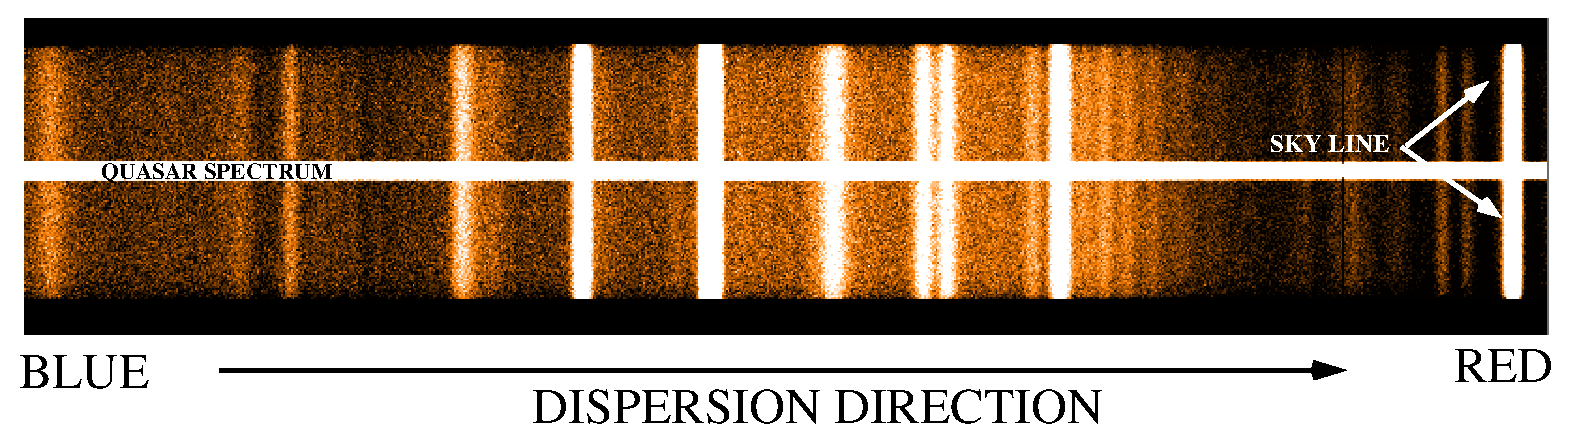
\psfig{file=spectrum_fig1.ps,width=16.0cm,angle=0}}
\caption{Two-dimensional quasar spectrum as displayed by {\sc gaia}}
\end{figure}

Display the other two spectra in new {\sc gaia} windows and familiarize yourself with them. The
arc spectrum should consist of a series of bright vertical emission
lines. These emission lines have known wavelengths, and will be used 
to wavelength calibrate the quasar spectrum (i.e. make the conversion 
between pixel coordinates and wavelength). The flatfield spectrum
should look fairly uniform (i.e pixel values $\simeq1$) and is
basically a map of the different sensitivity 
of the CCD pixels. By dividing the quasar spectrum by the flatfield 
it is possible to correct for this difference in sensitivity with wavelength.


{\large {\bf 4. Flatfielding}}\\
The first task is to flatfield the quasar spectrum, which simply involves
dividing the quasar spectrum by the flatfield spectrum. To do this we
use a {\sc iraf} task called {\it imarith}. From the {\sc iraf} command prompt type:

{\tt imarith quasar.fits \verb,/, flatfield.fits quasarflat.fits}

This should produce a new file called \verb,``quasar_flat.fits'', (you can
choose any name you like of course) in your home directory. To use
{\it imarith} to perform other arithmetic operations you simply
replace \verb,/, by \verb,+-*.,

{\large {\bf 5. Sky subtraction}}\\
At present the quasar spectrum contains the signal from the quasar
itself {\it plus} the spectrum of the night sky (including the bright
sky lines). The next stage of the reduction process is to remove the
night sky emission from the quasar spectrum, a process known as ``sky
subtraction''. To perform the sky subtraction you are going to use an
{\sc iraf} task called {\it background}. This task works by fitting a
polynomial function to the sky signal in each column of the
two-dimensional spectrum and then subtracting it. However, there is a
slight complication here, because along the middle of the
two-dimensional spectrum the quasar spectrum is superimposed on top of
the sky spectrum, and we don't won't to include this region in our sky
fit. This problem is illustrate in Fig 4, which shows a plot of the
flux in one column of the two-dimensional quasar spectrum. So, the
first task is to determine which range of y-pixel values in the
two-dimensional quasar spectrum are dominated by sky. Using {\sc gaia}
you should note down four y-pixel values which describe the
two regions of the two-dimensional spectrum which are dominated by sky
(i.e. $y_1 \rightarrow y_2$ and $y_3 \rightarrow y_4$).



Once you've done this you can subtract the sky-background by typing:

{\tt background quasarflat.fits quasarskysub.fits axis=2 sample= }$y_1:y_2,$ $y_3:y_4$


\begin{figure}
\centerline{\psfig{file=spectrum_fig2.ps,width=16.0cm,angle=0}}
\caption{Illustration of how the {\sc iraf} task {\it background}
subtracts the sky background from 2D spectra by fitting either side of
the object spectrum.}
\end{figure}

Make sure that you now have a new file in your home directory which is
the flatfielded quasar spectrum with the sky background removed.


{\large {\bf 6. Extracting the quasar spectrum }}\\
The next stage of the reduction process is to turn the two-dimensional
quasar spectrum into one-dimensional spectrum of flux versus
x-pixel. This process is know as {\it extracting} the spectrum and is
performed with an {\sc iraf} task called {\it apsum}. At the command
prompt, type:

{\tt apsum quasarskysub.fits}

(If you are asked how many apertures to identify, simply type: 1 $<$return$>$).
This will produce a file called ``quasarskysub.ms.fits'' which is your
one-dimensional spectrum. To extract the one-dimensional spectrum
{\it apsum} performs the following operation: at each x-pixel
position in the two-dimensional spectrum, {\it apsum} detects which y-pixels
are dominated by the quasar spectrum and simply adds the flux in those pixels
together. The final result of this process is a one-dimensional
spectrum of flux versus x-pixel value. The range of y-pixels dominated
by the quasar spectrum is referred to as the extraction {\it
aperture}, which explains why the task is called {\it apsum}.

At this stage you can take a first look at your one-dimensional quasar
spectrum using the {\sc iraf} task {\it splot} (spectra-plot). At the
command prompt type:

{\tt splot quasarskysub.ms.fits}

\newpage

As well as simply displaying spectra, the {\it splot} task allows you
to perform many basic analysis tasks (ask the demonstrator to show you
how it works).



{\large {\bf 7. Wavelength calibration}}
\begin{figure}
\centerline{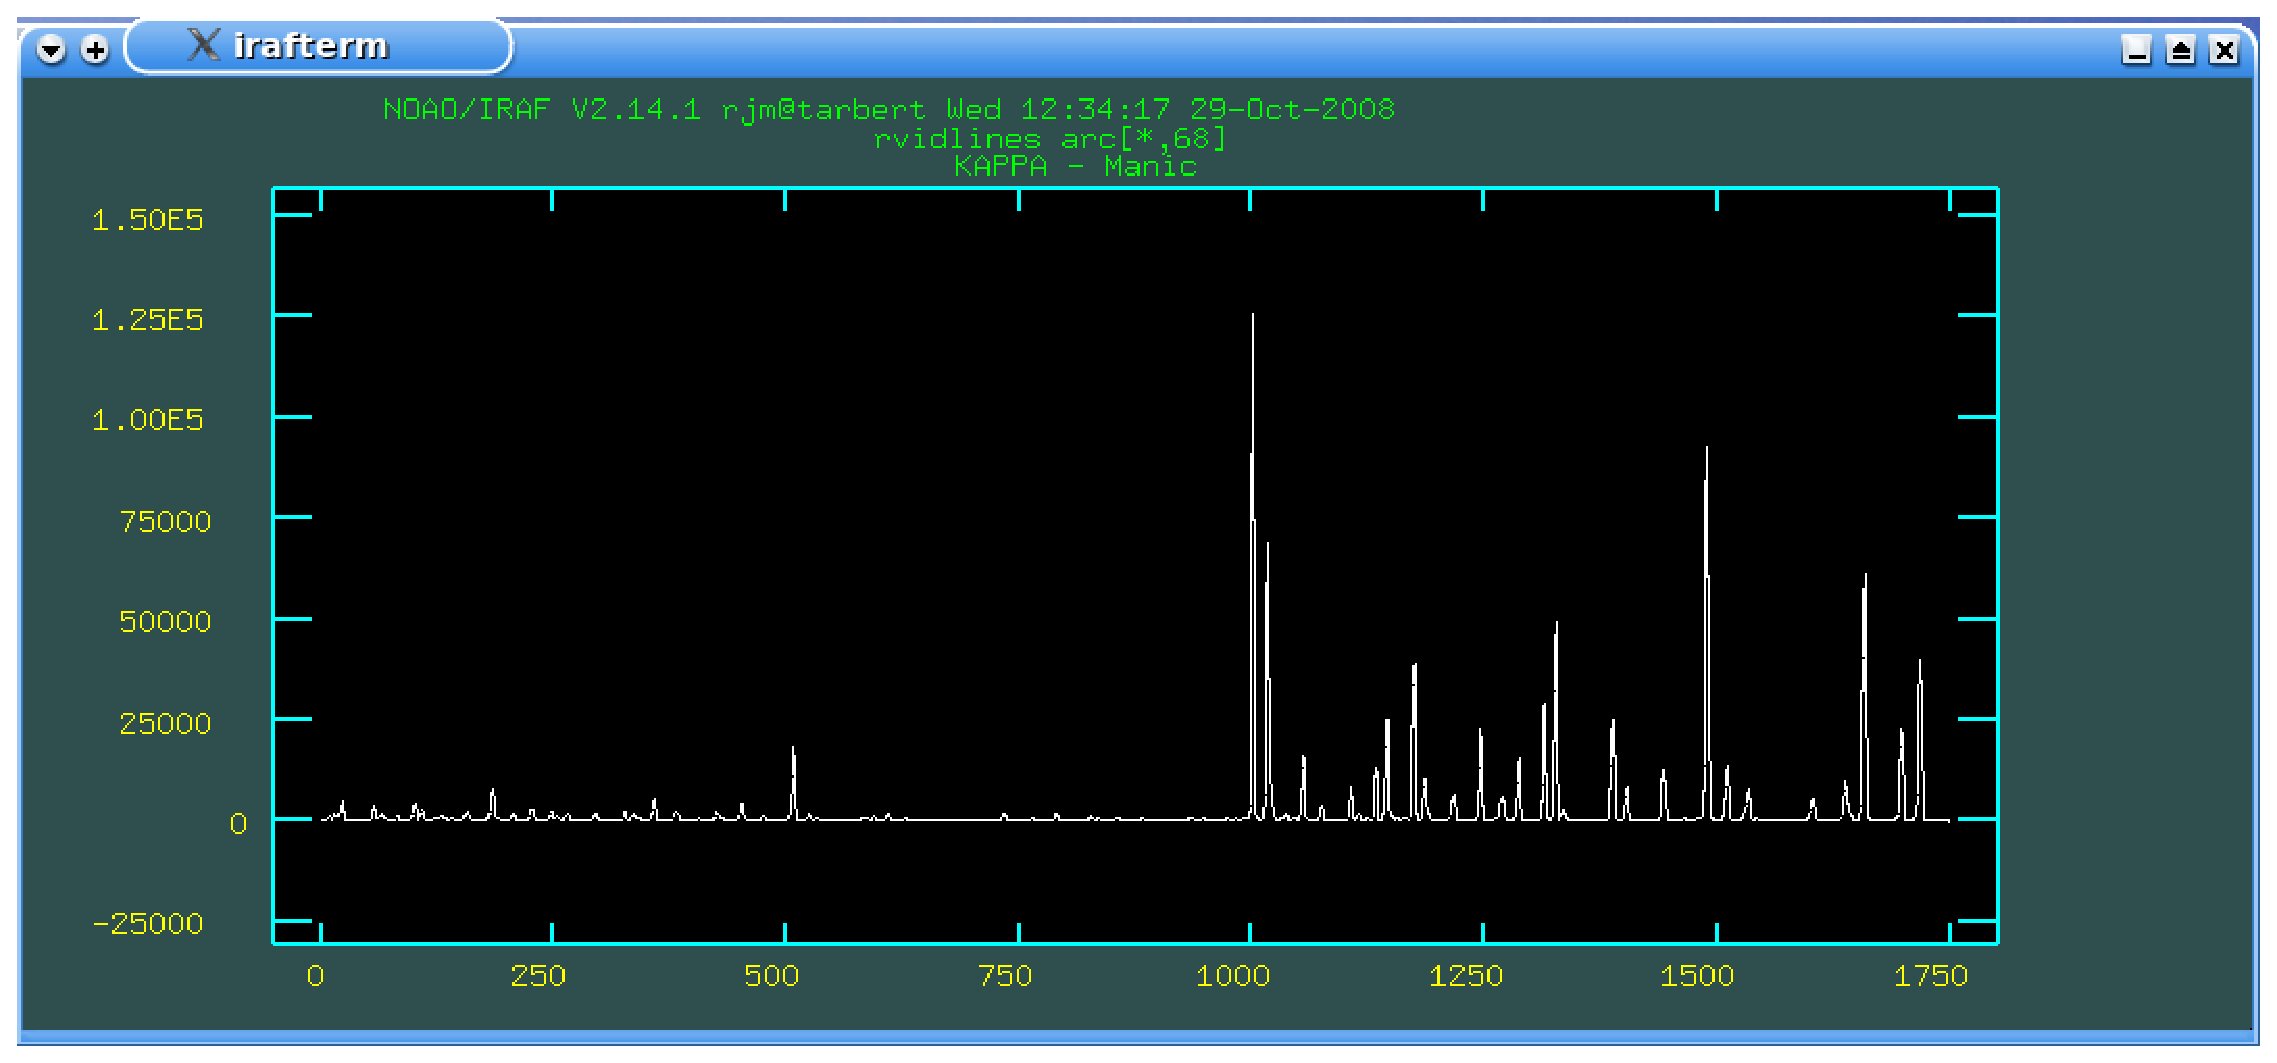
\psfig{file=arc.ps,width=16.0cm,angle=0}}
\caption{{\sc iraf} window generated by {\it identify} showing the
arc spectrum}
\end{figure}

The next stage in the reduction process is to perform the wavelength
calibration. At present, the one-dimensional spectrum of the quasar is
simply flux versus x-pixel number, and we need to
convert this into a one-dimensional spectrum of flux versus
wavelength. To achieve this we have to analyse a so-called ``arc
spectrum'', which is a spectrum of a gas discharge tube containing
elements\footnote{in this case helium, neon and argon} which produce emission lines at known laboratory
wavelengths. By studying the arc spectrum it is therefore possible to
perform the transformation between x-pixels and wavelength. The
wavelength calibration is performed using the {\sc iraf} task {\it
identify}. At the command prompt, type:

{\tt identify arc.fits}

Which should open a new window showing the arc spectrum (see Fig 5). 
In order to make the identification of the arc lines easier, it
may be worthwhile extending the new window horizontally (ask the
demonstrator how to do this).

Now for the tricky bit. You need to compare this arc spectrum with that
contained in the {\em CCD Atlas of Helium/Neon/Argon Spectra} (see Appendix\footnote{note: one of the 
arc lines has the wrong wavelength in the appendix}), 
in order that you can identify $\simeq 20$ lines of known wavelength, preferably
scattered reasonably well through the spectral range. 
It is a good idea to print out your arc spectrum, so that you can write
wavelengths on it for those lines that you believe you have identified.
As a clue, the bright line at pixel number 500 is the 5015.675 \AA\ line
which comes before a region of much weaker emission lines, and the bright
line at pixel number 1000 is the 5852.4878\AA\ line which comes at the red
end of this emission-line ``desert''. 


To identify the lines, click on the {\it identify} window to activate
it, place the cursor over the arc line of interest and press the ``m''
key to mark the line. At this point you will be asked to enter the
wavelength of the arc line. Repeat this process
until you have identified $\simeq20$ arc lines. Once you have
identified enough arc lines you can press ``f'' to fit the dispersion
solution. The {\it identify} window will update to show you the fit,
at which point you can delete outlier points with the ``d'' key and
re-fit the solution by pressing ``f'' once again. Once you are happy
with the quality of the fit (all points within $\simeq1$\AA\,) press
``q'' twice to exit {\it identify}, and then confirm that you want to 
write the dispersion solution to the database.

To let {\sc iraf} know that you want to associate this dispersion
solution with your one-dimensional quasar spectrum, type:

{\tt hedit quasarskysub.ms.fits fields=REFSPEC1 value=arc.fits}

And finally, to apply the wavelength calibration to your quasar
spectrum, type:

{\tt dispcor quasarskysub.ms.fits \verb,quasarskysub_wave.ms.fits,}


{\large {\bf 8. Redshift determination}}

You can now view your final wavelength calibrated spectrum by typing:

{\tt splot \verb,quasarskysub_wave.ms.fits,}

Using {\it splot} note down the wavelengths of any obvious emission
lines in the quasar spectrum using the cursor and by pressing the space bar.

\bigskip

Redshift $z$ is defined by the equation

$$\lambda_{observed} = (1 + z) \lambda_{emitted}$$

and so if you can work out which emission lines these actually are, then
it is trivial to calculate the redshift. Moreover, you will know if
you have identified the emission lines correctly because then 
the calculation of redshift from each emission line will give the same
value of $z$ to an accuracy of typically 3 decimal places.

A list of the brightest emission lines seen in active galaxies and
quasars is given below, along with their laboratory wavelengths. 
Only a few of these lines are ever visible in the optical spectrum of a given quasar, and
precisely which ones are visible obviously depends on its actual redshift.
 
By a process of elimination, work out which of these lines are visible in
your reduced spectrum, and hence calculate the redshift of the quasar,
quoting an accuracy based on the line-by-line variation in $z$. {\bf It is important that
you clearly demonstrate in your report how you determined the quasar redshift.}

\newpage

{\large {\bf 9. Saving plots for your report}}\\
For the purposes of writing your final report you may want to include
plots of the various stages of the reduction process. For capturing
screenshots of any window the easiest thing is probably to use the
software package {\it xv} which is started by simply typing:

{\tt xv} 

in a terminal window. 


Within {\sc iraf} you can generate
postscript copies of the plots generated by {\it splot, identify} etc
by typing:

{\tt :.snap eps}

in the appropriate window. This will produce a postscript ``.eps''
copy of the {\sc iraf} window in your directory which can be viewed
with ghostview (gv) and then printed.



{\bf Table: Prominent UV/optical emission lines in quasars}

\begin{tabbing}

Lyman $\alpha$  \hspace*{2cm} \=  1215\AA \\

NV          \>      1240\AA \\

CIV         \>      1549\AA \\

CIII        \>      1909\AA \\

MgII        \>      2799\AA \\

HeI         \>      3189\AA  \\ 

[NeV]        \>     3426\AA  \\

[OII]     \>      3728\AA \\

[NeIII]    \>     3870\AA \\

[NeIII]    \>     3961\AA \\

H$\delta$ \>      4103\AA \\

H$\gamma$ \>      4346\AA \\

H$\beta$    \>      4861\AA \\

[OIII]    \>      4959\AA \\

[OIII]    \>      5007\AA \\

[OI]      \>      6300\AA \\

H$\alpha$   \>      6563\AA \\

[SII]     \>      6724\AA \\


\end{tabbing}

\newpage

\pagestyle{myheadings}
\markboth{Astrometry}{Astrometry}
\renewcommand\baselinestretch{1.0}
\setcounter{page}{1}
\begin{center}
{\Huge \bf Astrometry}
\end{center}

Astrometry is the determination of accurate spherical coordinates, Right Ascension\,($\alpha$) and Declination\,($\delta$), for an object whose position was previously either unknown or poorly established. As well as simply establishing the position of astronomical sources, astrometry can be used to measure the proper motion of objects such as asteroids or `nearby' stars, provided astronomical images at suitably different  epochs are available. 

In fact, asteroids move sufficiently quickly that they produce a trail across a long exposure CCD image. Measurement of the length of this trail can thus be used to establish the proper motion of the asteroid.

The aim of this exercise is to measure the proper motion of the \setcounter{page}{1}13th-magnitude asteroid (595) Polyxena from its trailed image on a 90-minute CCD exposure and hence to estimate its orbital radius from the sun.

\begin{enumerate}

\item The position of the beginning and end of the asteroid trail needs to be established by setting up a coordinate frame\,(known as a plate solution) fitted to the measured $x,y$ positions of stars of known $\alpha$ and $\delta$ which can be seen on the CCD image around the position of Polyxena. The first thing you therefore need to do is to load the {\tt polyxena.fits} CCD image into {\sc gaia} and measure the $x,y$ coordinates of the 25 stars shown in Fig. 6. The stars are numbered, and their equatorial coordinates are provided in Table 1, so make sure you note down which $x,y$ coordinate refers to which star. 

\item You should now have all the information necessary to make a final list containing 5 columns: star number, $\alpha$, $\delta$, x, y. Based on this list you can now use {\sc gaia} to perform the coordinate transformation\,(ask your demonstrator to help with this). Using the grid of 25 stars, it should be possible to produce a plate solution with a rms of $\simeq 0.5$ arcseconds. When you have an good solution, accept the fit and save the {\tt polyxena.fits} image under a new filename (e.g. {\tt polyxena-astrom.fits}). Reload this new image into {\sc gaia} and carefully measure the ($\alpha$, $\delta$) coordinates of the start and end of the asteroid trail\,(which can be seen near the centre of the field of view).

\item Based on the coordinates of the start and end of the asteroid trail\,(and the 90 minute exposure time), it is now possible to calculate the angular velocity of the asteroid\,({\bf think about the cos($\delta$) factor!}). Assuming circular motion for the asteroid's orbital path around the Sun, and knowing that the field was close to opposition at the time of observation\,(see Appendix), compute its distance from the Sun in Astronomical Units. As indicated by the diagram, you can assume that
the asteroid is orbiting the Sun in the same direction as the Earth.

\end{enumerate}

\newpage

\begin{figure}
\centerline{\psfig{file=stars.ps,width=18.0cm,angle=0}}
\caption{Screenshot of the polyxena.fits image showing the locations of the 25 stars which can be used to define the equatorial coordinate system.}
\end{figure}

\newpage

\begin{table}
\begin{center}
\begin{tabular}{|r|l|l|}
\hline
  \multicolumn{1}{|c|}{Star} &
  \multicolumn{1}{c|}{RA} &
  \multicolumn{1}{c|}{Dec} \\
\hline
  1 & 14:52:49.429 & $-$28:54:51.13\\
  2 & 14:52:40.927 & $-$28:56:37.55\\
  3 & 14:51:52.970 & $-$28:58:56.30\\
  4 & 14:51:51.318 & $-$28:59:00.21\\
  5 & 14:52:14.225 & $-$29:02:41.80\\
  6 & 14:52:06.541 & $-$29:03:31.15\\
  7 & 14:51:44.912 & $-$29:02:41.68\\
  8 & 14:52:02.075 & $-$29:05:46.92\\
  9 & 14:52:05.628 & $-$29:11:02.29\\
  10 & 14:52:02.219 & $-$29:12:39.20\\
  11 & 14:52:35.570 & $-$29:09:41.13\\
  12 & 14:53:04.314 & $-$29:05:43.35\\
  13 & 14:53:07.746 & $-$29:04:42.56\\
  14 & 14:51:00.138 & $-$28:58:57.20\\
  15 & 14:50:53.009 & $-$29:00:13.11\\
  16 & 14:51:07.926 & $-$29:12:56.19\\
  17 & 14:52:56.981 & $-$28:59:47.82\\
  18 & 14:52:50.848 & $-$29:01:58.89\\
  19 & 14:52:48.953 & $-$29:03:11.91\\
  20 & 14:52:44.232 & $-$29:03:59.56\\
  21 & 14:52:42.356 & $-$29:05:36.85\\
  22 & 14:51:25.420 & $-$29:08:48.12\\
  23 & 14:51:16.278 & $-$29:06:31.77\\
  24 & 14:51:10.221 & $-$29:08:07.60\\
  25 & 14:51:07.936 & $-$29:06:44.75\\
\hline\end{tabular}
\caption{List of equatorial coordinates for the 25 stars highlighted in Fig. 6}
\end{center}
\end{table}

%\vspace*{2cm}
%{\bf Data for the film/plate used}:\\
%UKST original plate J1494, Field 448, centre 14$^h$ 57$^m\:\: -30^{\circ}$\\
%Plate scale: 67.12 arcsec per mm\\
%Date of observation: 1975 May 17, LST at start of exposure 14$^h$ 46$^m$\\
%Exposure duration: 90$^m$
%RA of Sun on May 17: 3$^h$ 33$^m$\\

%{\bf See}:\\
%KOWAL: Asteroids, their Nature and Utilization (ROE Library
%523.44(02.063))\\
%Ephemerides of Minor Planets 1975 (ROE Library).


%\newpage

%\scalebox{0.9}{\includegraphics{ap3labman_astrom1.ps}}

%\newpage

%\scalebox{0.9}{\includegraphics{ap3labman_astrom2.ps}}

%\newpage

%\scalebox{0.9}{\includegraphics{ap3labman_astrom3.ps}}

%\newpage

%\scalebox{0.9}{\includegraphics{ap3labman_astrom4.ps}}

\newpage

\pagestyle{empty}

\vspace{2cm} 






\centerline{\hspace{-2cm}  \Huge APPENDIX 1}

\vspace{4cm} 


\centerline{\Large \hspace{-1cm} A CCD atlas of Helium/Neon/Argon spectra}

\vspace{1cm} 


\centerline{\hspace{-1cm} E. Carder (April 17, 1996)}


\newpage


\scalebox{0.85}{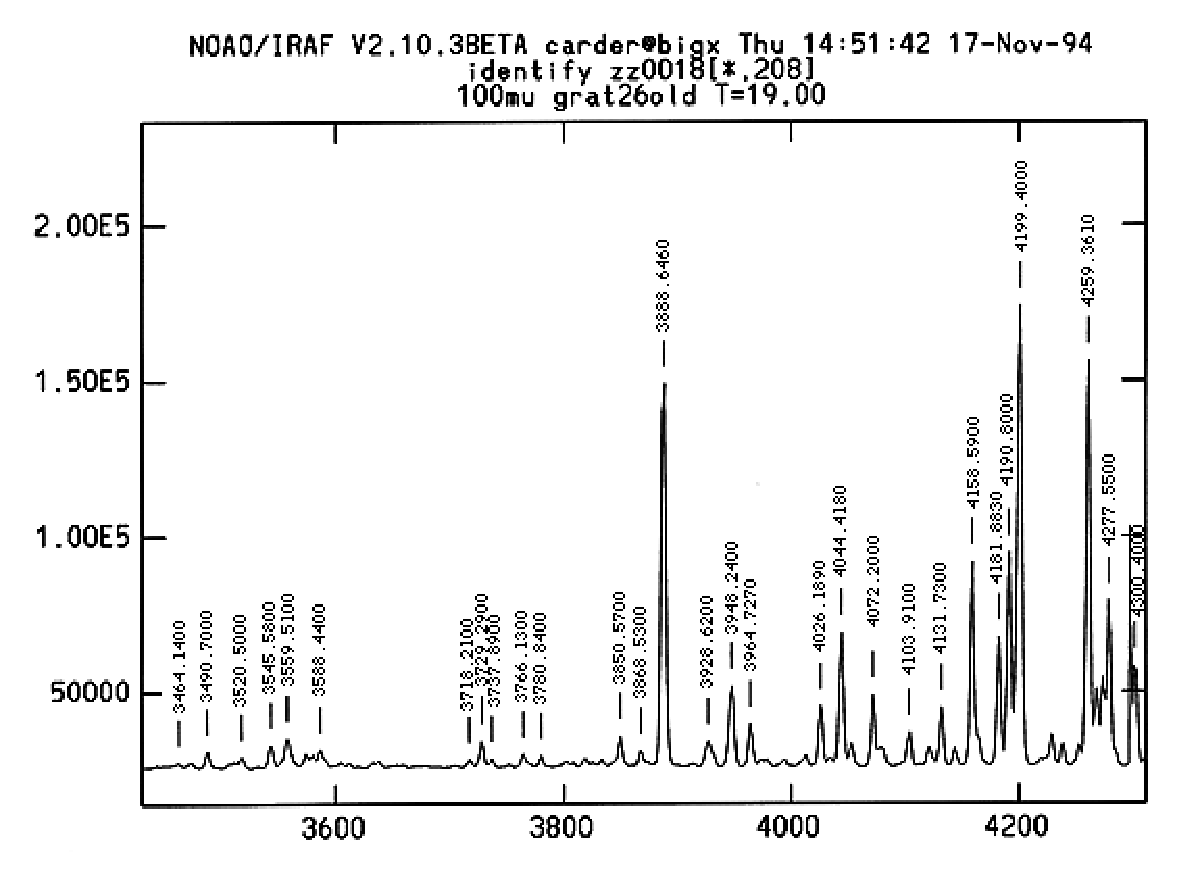
\includegraphics{spec0.ps}}

\scalebox{0.85}{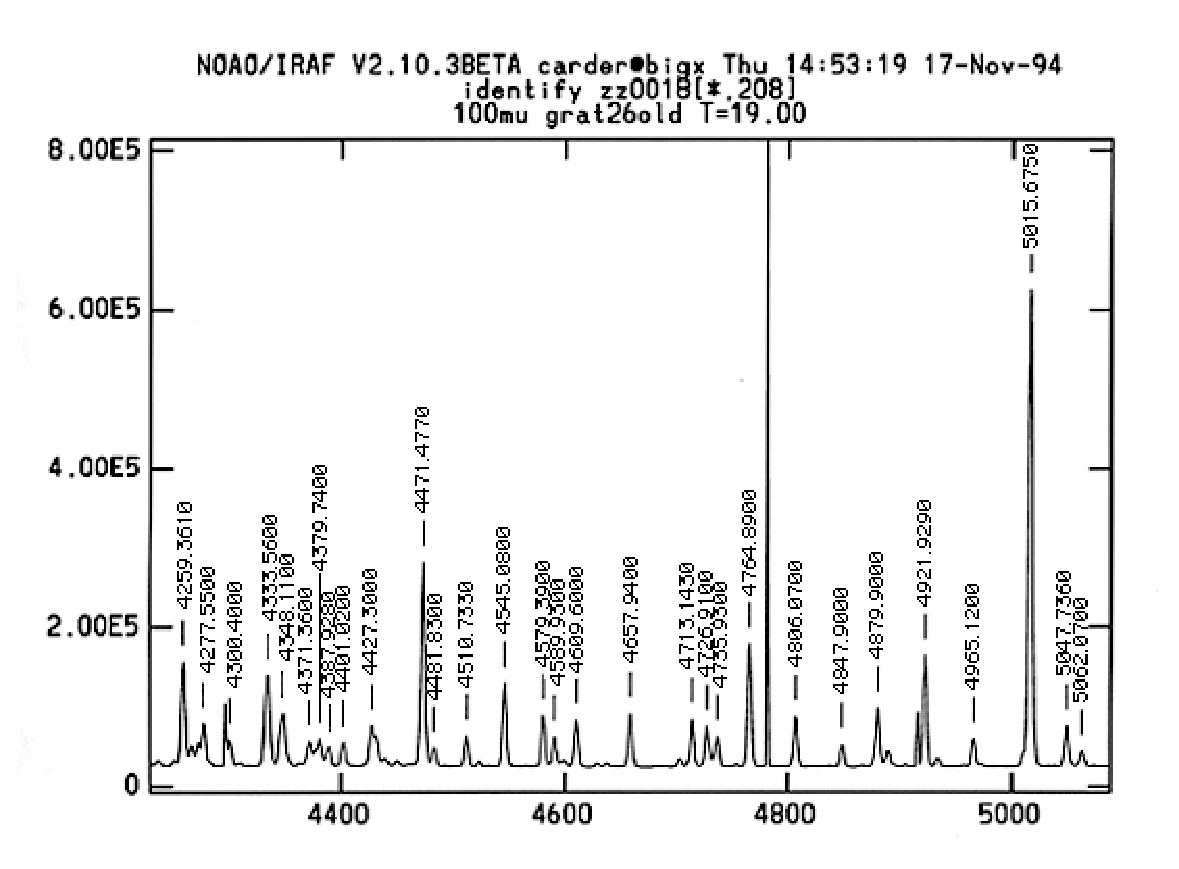
\includegraphics{spec1.ps}}
\scalebox{0.85}{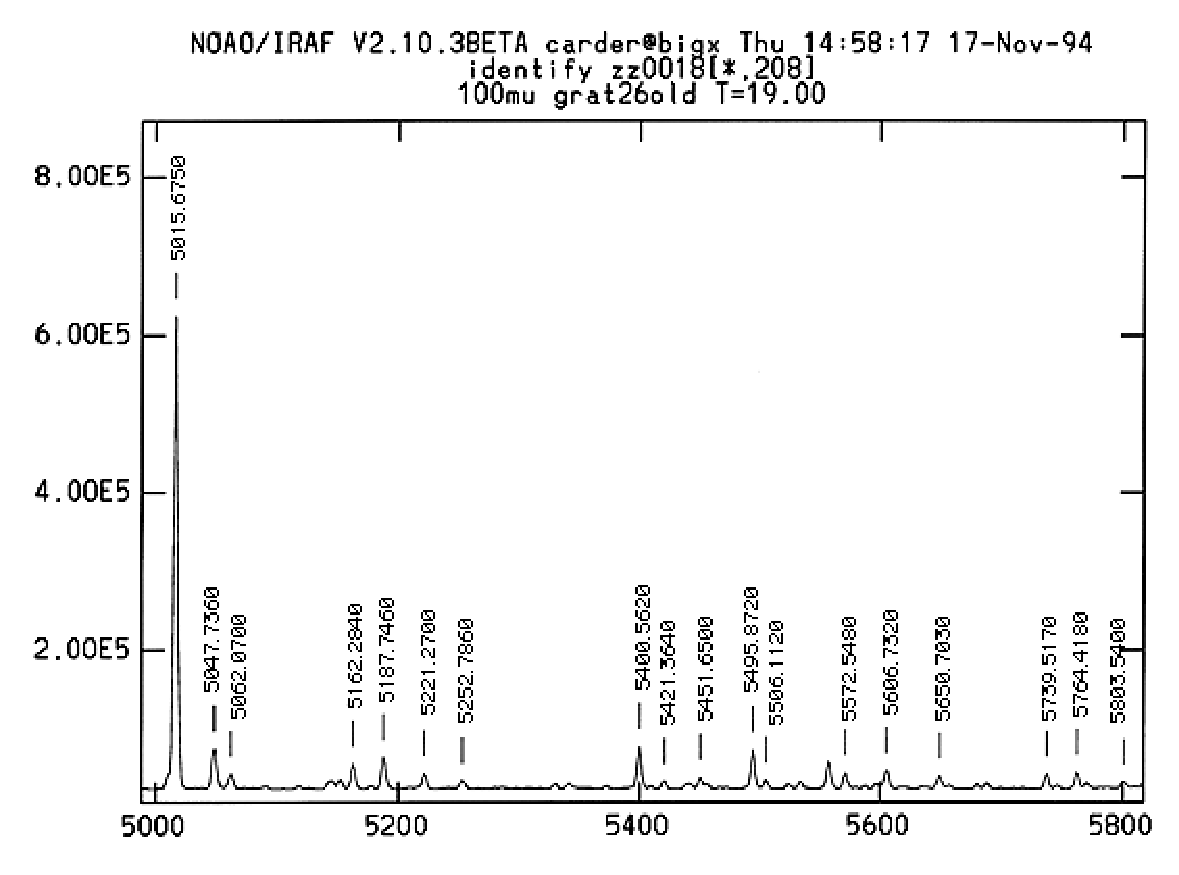
\includegraphics{spec2.ps}}
\scalebox{0.85}{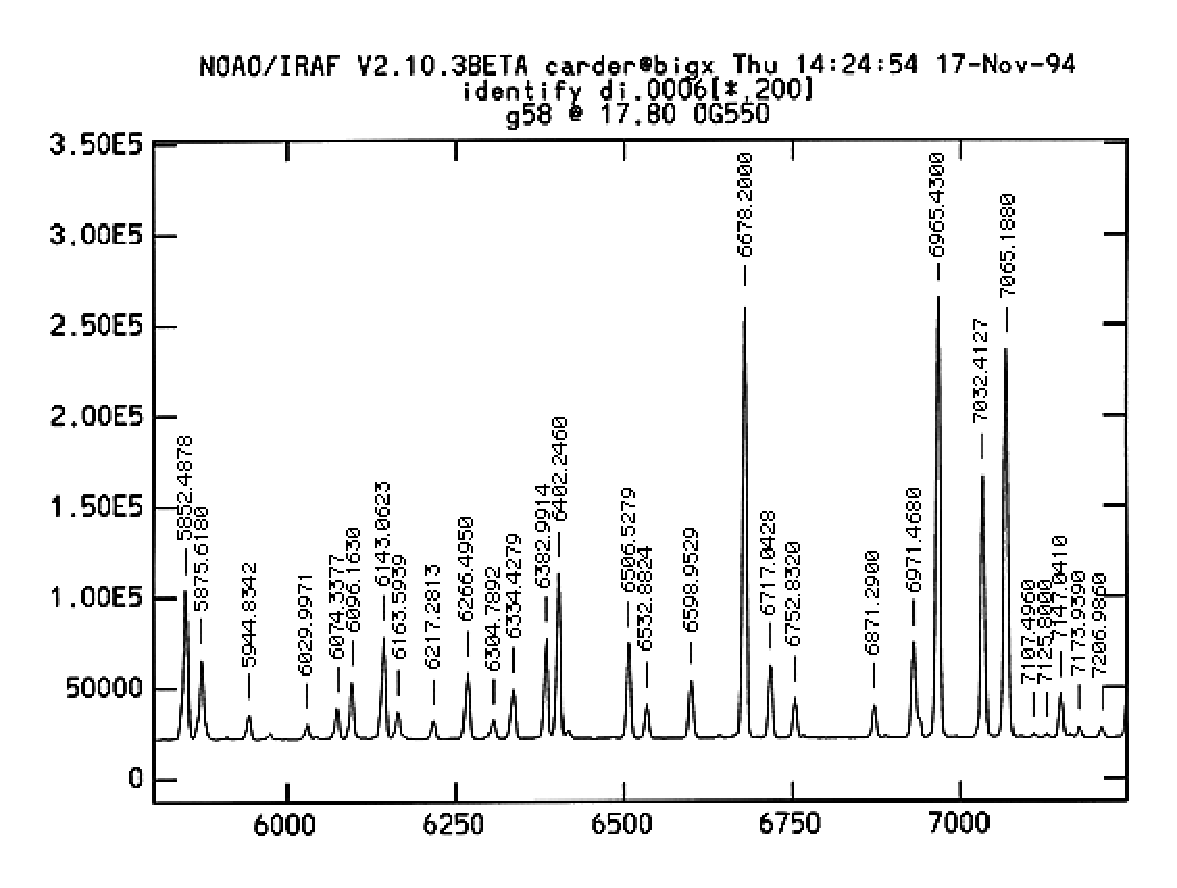
\includegraphics{spec3.ps}}
\scalebox{0.85}{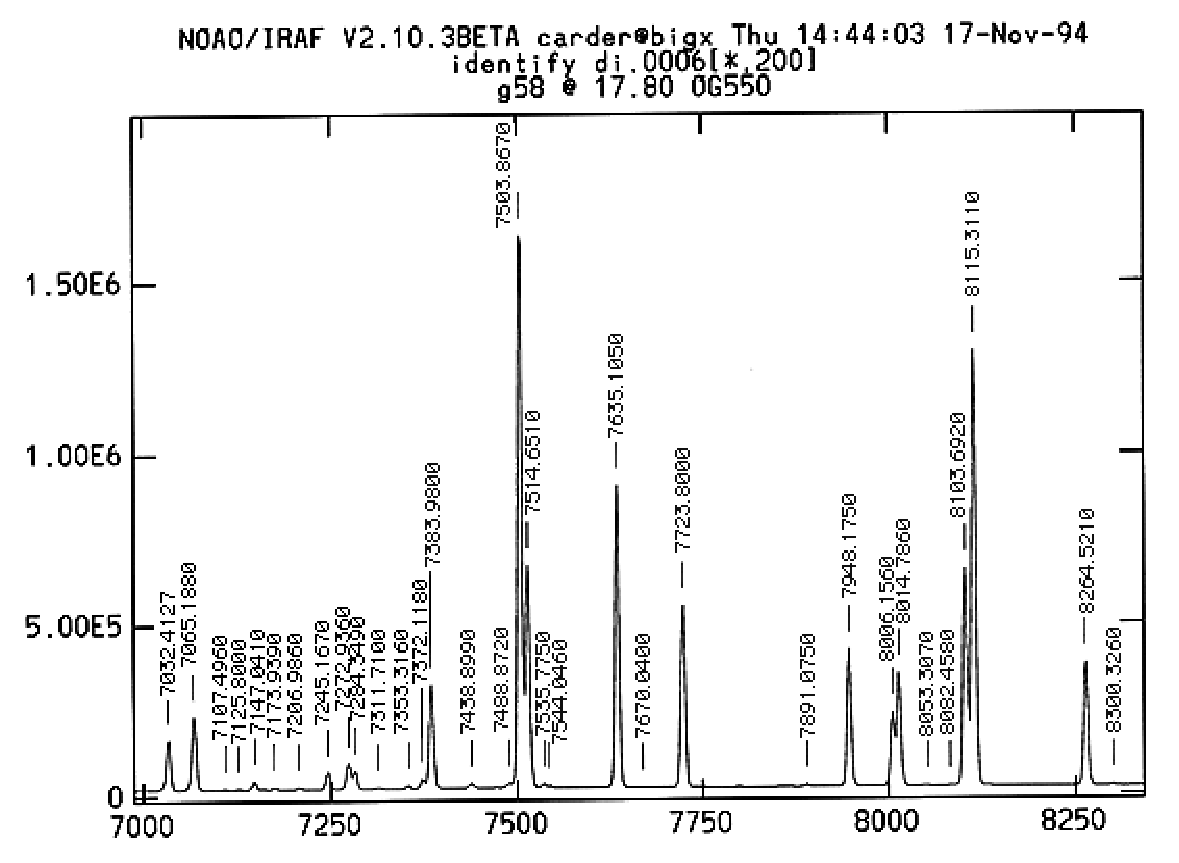
\includegraphics{spec4.ps}}
\scalebox{0.85}{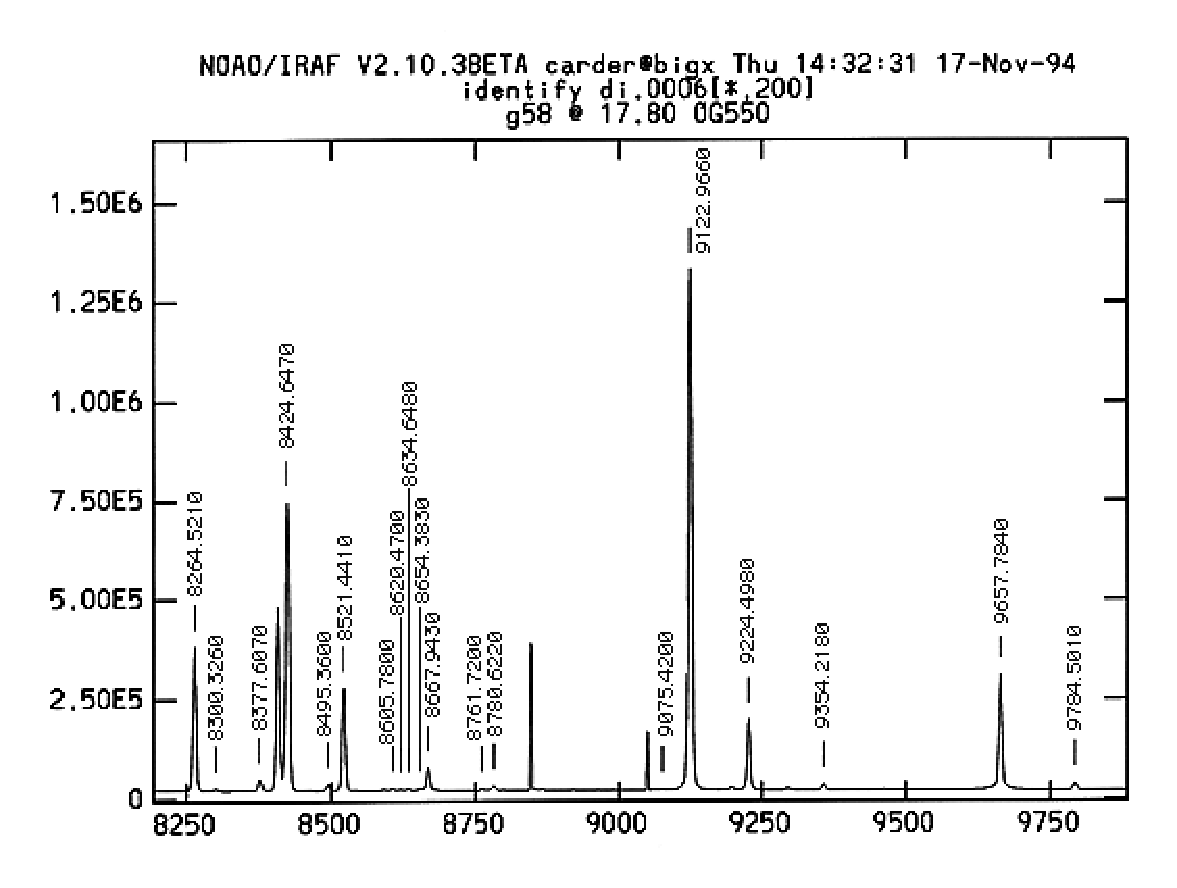
\includegraphics{spec5.ps}}




\newpage

\pagestyle{empty}

\vspace{2cm} 

\centerline{\Huge APPENDIX 2}

\vspace{2cm}

\leftline{\Large Basic Unix Commands}



\begin{table}[h]
\begin{tabular}{lll}
\hline
Command&&Description\\
\hline
cd                &&  Change location to home directory\\
cd dirname        &&  Change location to directory dirname\\
cd ..             &&  Move up one directory in the tree\\
pwd               && Print current directory\\
ls                && List files in current directory\\
ls -l             && List files in detail\\
more f1           && Show contents of f1 on the screen\\
mkdir dirname     &&  Create new directory dirname\\
rmdir dirname     &&  Remove directory dirname\\
mv f1 dirname     && Move file f1 to directory dirname\\
mv f1 f2          && Rename file f1 as f2\\
cp f1 dirname     && Copy file f1 to directory dirname\\
cp f1 f2          && Copy file f1 to new file f2\\
rm f1             && Remove file f1\\
exit              && Close current terminal window\\
passwd            && Change password\\
\hline
\end{tabular}
\end{table}

\medskip 

\leftline{\Large Useful software packages}

For working with ascii data files on the Unix system it is probably
easiest to use the basic text editor package: {\it emacs}. To open a new
file with emacs, simply type at the command prompt:

{\tt emacs myfile.txt (return)}

For grabbing screenshots and converting images between different
formats, a useful software package on the Unix system is {\it xv}. To
launch xv just type at the command prompt:

{\tt xv (return)}

For viewing and printing postscript files, use the software package
{\it gv}. At the command prompt type:

{\tt gv (return)}

For plotting graphs and fitting functions the easiest package to use
if probably {\it gnuplot}. On the next page there is a brief tutorial
on how do use gnuplot.


\newpage
\centerline{\Huge APPENDIX 3}

\begin{center}
{\large{\bf Gnuplot}}
\end{center}
This is designed to be a very brief tutorial on using the plotting
package Gnuplot. More information can be found at: {\tt
http://www.gnuplot.info/}, and a more detailed tutorial can be found
at: {\tt http://www.duke.edu/~hpgavin/gnuplot.html}.

Start Gnuplot by simply typing:

{\tt gnuplot -mono (return)}

on the command line. In your home directory I have included a file
called {\tt toydata.dat} to illustrate how the basic features of
Gnuplot work. This file contains three columns: x, y \& y error. 
To simply plot x versus y, type:

{\tt gnuplot> plot ``toydata.dat''}

Gnuplot should produce a plot of x versus y in a new window, and will
automatically choose appropriate ranges for the x-axis and y-axis. To
label the axes and to add a title type:

{\tt gnuplot> set xlabel ``x''}\\
{\tt gnuplot> set ylabel ``y''}\\
{\tt gnuplot> set title ``toydata plot''}

If you now type:

{\tt gnuplot> plot ``toydata.dat''}

The graph should be correctly labelled. To plot the data including the
errors on the y variable you can type:

{\tt gnuplot> plot ``toydata.dat'' with yerrorbars}

To fit a function to your data-set you can type:

{\tt gnuplot> f1(x)=a*x+b}

which defines a new linear function (gnuplot can fit much more
complicated functions if necessary). And then type:

{\tt gnuplot> fit f1(x) ``toydata.dat'' using 1:2 via a,b}

which tells Gnuplot to fit the function to columns 1 \& 2 of
``toydata.dat'', determining the best-fitting values of parameters a
\& b. To then produce a combined plot of your data and the best-fitting
function you can type:

{\tt gnuplot> plot ``toydata.dat'' with yerrorbars, f1(x)}\\
\newpage
At the end of this process the graph in the Gnuplot window should look
something like Fig 1. If you wanted to save your graph as a postscript
file (suitable for printing) you could type:

{\tt gnuplot> set terminal postscript landscape}\\
{\tt gnuplot> set output ``toydataplot.ps''}\\
{\tt gnuplot> plot ``toydata.dat'' with yerrorbars, f1(x)}\\
{\tt gnuplot> set terminal x11}

which should produce a postscript file called ``toydataplot.ps''. The
final command returns the default output to the normal Gnuplot
window. To exit Gnuplot type {\tt CNTR-D}.

\begin{figure}
\centerline{\psfig{file=toydataplot.ps,width=14.0cm,angle=270}}
\caption{Example graph produced 
by gnuplot based on the datafile ``toydata.dat'.}
\end{figure}

\newpage

\centerline{\Huge APPENDIX 4}

\Large{Error Propagation:}\\

\bigskip

\noindent
Addition/Subtraction: If $f=a\pm b$, then $\sigma_f$ is given by:
\begin{center}
\Large {$\sigma^2_{f} = \sigma_a^2 + \sigma_b^2$}
\end{center}

\bigskip

Multiplication/Division: if $f=ab$ or $f=a/b$, then $\sigma_f$ is
given by:
\begin{center}
\Large{$\left(\frac{\sigma_f}{f}\right)^2 = \left(\frac{\sigma_a}{a}\right)^2 + \left(\frac{\sigma_b}{b}\right)^2$}
\end{center}

\bigskip

Raising to a power: If $f=a^c$, where $c$ is a constant, then
$\sigma_f$ is:
\begin{center}
\Large{$\frac{\sigma_f}{f}=c\left(\frac{\sigma_a}{a}\right)$}
\end{center}

\bigskip

Logarithms: If $f=\log_{e}(a)$ then $\sigma_f$ is given by:
\begin{center}
\Large{$\frac{\sigma_f}{f}=\frac{1}{a}$}
\end{center}
Remember that: $\log_{e}(a)=\log_{e}(10)\times \log_{10}(a)$




\end{document}



